% Ltex language=en
% \documentclass[12pt, 1p, review, number]{elsarticle}
\documentclass[3p,twocolumn,preprint]{elsarticle}
%\documentclass[10pt,a4paper,3p,twocolumn]{elsarticle}
% \documentclass[5p,preprint,twocolumn]{elsarticle}
%----------------------------------------------------------------------
%                     Loading of packages
%----------------------------------------------------------------------

% for cutting words
\usepackage[utf8]{inputenc}
% a font close to that chosen by Elsevier
\usepackage[bitstream-charter]{mathdesign}
\usepackage{mathtools, cuted}
% for accentuated characters
%\usepackage[T1]{fontenc}
\geometry{top=2cm,left=1.5cm,bottom=2cm,right=1.5cm}
\usepackage{multicol}
% For treating ps:
\usepackage{psfrag}
% For subfigures

\usepackage{subcaption}
\usepackage{placeins}
% For tables
\usepackage{array}
\usepackage{multirow}
\usepackage{hhline}
\usepackage{colortbl}
\usepackage{tabulary}
\usepackage{etoolbox}
% For citations
\usepackage[numbers]{natbib}
%\biboptions{longnamesfirst,angle,semicolon}
%\citetstyle{nature}
% For color
\usepackage{color}
\usepackage{xcolor}
% For spacing
\usepackage{setspace}
%\doublespacing
\singlespacing
%\onehalfspacing
% For maths
\usepackage{amsmath, amsfonts}
\usepackage[squaren,ashgrey]{SIunits}
% For Line numbering
\usepackage[pagewise,modulo]{lineno}
%\linenumbers
% For special characters
\usepackage{pifont}
%
\usepackage[pagebackref,colorlinks=True]{hyperref}
\usepackage{wasysym}
\usepackage{color}
\usepackage{cleveref}
\crefformat{figure}{(Fig.~#2#1#3)}
\usepackage{hyperref}
\usepackage[hyperpageref]{backref}
\usepackage{lipsum}
\usepackage{booktabs} % To thicken table lines
% \usepackage{widetext}
\usepackage{float}
\usepackage{empheq}
\usepackage{graphicx}
%\usepackage{siunitx}


%----------------------------------------------------------------------
%                     Commands
%----------------------------------------------------------------------
\renewcommand*{\overrightarrow}[1]{\vbox{\halign{##\cr \tiny\rightarrowfill\cr\noalign{\nointerlineskip\vskip1pt}$#1\mskip2mu$\cr}}}
%% Degree character
\DeclareTextSymbol{\degr}{T1}{6}
\newcommand{\degre}[0]{\degr C}
\DeclareUnicodeCharacter{2212}{-}
% MPam^0.5 character
\newcommand{\mpa}[0]{\mbox{MPa}\sqrt{\mbox{m}}}
%mettre de nouilles sous les tenseurs
\newcommand{\ve}[1]{{\underline{#1}}}
\def\ten#1{\oalign{$#1$\crcr\hidewidth$\scriptscriptstyle\sim$\hidewidth}} 
% derivee seconde
\newcommand{\fda}[2]{\displaystyle \frac{\partial\,{#1}}{\partial\, {#2}}}
% et al. for citations
\newcommand{\etal}[0]{{\em et al.}}
\renewcommand*\contentsname{\large{Table of contents}}
\def \hfillx {\hspace*{ -\linewidth} \hfill} % remplir espacement horizontal entre deux sous-figures de façon à remplir toute la largeur du texte.
%----------------------------------------------------------------------
%                     Colors
%----------------------------------------------------------------------
\definecolor{ashgrey}{rgb}{0.7, 0.75, 0.71}
%----------------------------------------------------------------------
%                     Pre-Document
%----------------------------------------------------------------------
\journal{Applied Energy}
%----------------------------------------------------------------------
%                     Document
%----------------------------------------------------------------------
\begin{document}

% \tableofcontents

\begin{frontmatter}

%% Title, authors and addresses

%% use the tnoteref command within \title for footnotes;
%% use the tnotetext command for theassociated footnote;
%% use the fnref command within \author or \address for footnotes;
%% use the fntext command for theassociated footnote;
%% use the corref command within \author for corresponding author footnotes;
%% use the cortext command for theassociated footnote;
%% use the ead command for the email address,
%% and the form \ead[url] for the home page:
%% \title{Title\tnoteref{label1}}
%% \tnotetext[label1]{}
%% \author{Name\corref{cor1}\fnref{label2}}
%% \ead{email address}
%% \ead[url]{home page}
%% \fntext[label2]{}
%% \cortext[cor1]{}
%% \address{Address\fnref{label3}}
%% \fntext[label3]{}

\title{Toward a novel piezoelectric energy harvester for earcanal dynamic motion exploitation, using a bistable resonator cycled by coupled hydraulic valves made of collapsed flexible tubes}

%% use optional labels to link authors explicitly to addresses:
%% \author[label1,label2]{}
%% \address[label1]{}
%% \address[label2]{}


\address[symme]{Laboratoire SYMME - Université Savoie Mont Blanc, 7 Chemin de Bellevue, 74940, Annecy}
\address[critias]{Université du Québec - École de technologie supérieure, Montréal, QC, H3C 1K3}


\author[symme]{Tigran AVETISSIAN}
\author[symme]{Fabien FORMOSA}
\author[symme]{Adrien BADEL}

%\author[critias]{Michel DEMUYNCK}
\author[critias]{Aidin DELNAVAZ}
\author[critias]{Jérémie VOIX}


\begin{abstract}
Scavenging energy from the earcanal's dynamic motion during jaw movements may be a practical way to enhance the battery autonomy of hearing aids. The main challenge consists in optimizing the amount of energy extracted while working with soft human tissues and the earcanal restricted volume. This paper proposes a new energy harvester concept: a liquid-filled earplug which transfers energy outside the earcanal to a generator. The latter is composed of a hydraulic amplifier, two hydraulic cylinders that actuate a bistable resonator to raise the source frequency while driving an amplified piezoelectric transducer to generate electricity. The cycling of the resonator is achieved using two innovative flexible hydraulic valves based on the buckling of flexible tubes.\\
A multiphysics-coupled model is established to determine the system operation requirements and to evaluate its theoretical performances. This model exhibits a theoretical energy conversion efficiency of 85\%. The electromechanical performance of the resonator coupled to the piezoelectric transducer, as well as the hydraulic behavior of the valves are experimentally investigated. The global model was updated using the experimental data to improve its predictability toward further optimization of the design. Moreover, the energy losses are identified to enhance the entire proposed design and improve the experimental energy conversion efficiency to 26\%.
\end{abstract}

\begin{keyword}
Energy harvesting, frequency-up, earcanal, multiphysics, hydraulic valve
\end{keyword}

\end{frontmatter}

%\linenumbers

%% main text
 % Ltex language=en
\begin{table*}
\begin{large}
	\begin{center}
		Nomenclature	\\
		\noindent\makebox[\linewidth]{\rule{\textwidth}{0.4pt}}
	\end{center}
\end{large}		
% \end{table*}
\begin{minipage}{.5\textwidth}
%%%%%%%%%%%%%%%%%%%%%%%%%%%%%%%%%%%%%%%
% \begin{table}[!h]
	\begin{tabular}{ c  m{6cm} }
		\textbf{Subscripts}      &                                                         \\
		APG                      & Amplified piezoelectric generator                       \\
		BB                       & Buckled beam                                           \\
		BR                       & Bistable resonator                                      \\
		GB                       & Guide beam                                             \\
		EH                       & Energy harvester                                        \\
		HA                       & Hydraulic amplifier                                     \\
		HC                       & Hydraulic cylinder                                      \\
		HV                       & Hydraulic valve                                         \\
		PFF						 & piezoelectric force factor  \\
		\textbf{Roman letters}   &                                                         \\
		$a$ [m]                  & HV bending lever arm                                    \\
		$a_h$ [-]                & Hydraulic amplification level                           \\
		$Cf$ [Pa.s$^2$.m$^{-6}$]         & Pressure loss coefficient                               \\
		$Cf_0$ [Pa.s$^2$.m$^{-6}$]       & Opened HV pressure loss coefficient                     \\
		$Cf_c$ [Pa.s$^2$.m$^{-6}$]       & Closed HV pressure loss coefficient                     \\
		$C_p$ [F]                & APG internal capacity                                   \\
		$D_h$ [m]                & Hydraulic diameter of the HV                            \\
		$D_{hc}$ [m]             & Hydraulic cylinder internal diameter                    \\
		$D_r$ [m]                & HV rigid sheath diameter                                \\
		$E_d$ [J]                & Global dissipated energy                                \\
		$E_e$ [J]                & Harvested electric energy                               \\
		$E_{hyd}$ [J]            & Available hydraulic energy from earplug                 \\
		$F_{br}$ [N]             & BR counter reaction force                               \\
		$f_0$ [Hz]				 &	BR natural resonance frequency						   \\
		$f_d$ [-]                & Dry friction loss coefficient                           \\
		$K$ [N/m]                & APG stiffness                                           \\
		$K_{bb}$ [N/m]           & 8 BB's stiffness                                        \\
		$K_{eq}$ [N/m]           & Equivalent stiffness seen from the APG                  \\
		$K_{gb}$ [N/m]           & GB stiffness                                            \\
		$K_{HV}$ [N.m/rad]        & HV stiffness                                            \\
		$K_s$ [N/m]              & Spring stiffness                                        \\
		$K_{\varphi}$ [N.m/rad]   & Single hinge stiffness                                  \\
		$k^2$ [-]                & APG electromechanical coupling coefficient              \\
		$k_{sys}^2$ [-]          & Global electromechanical coupling coefficient           \\
		$L$ [m]                  & Distance between 2 BR adjacent hinges on $\vec{x}$ axis \\
		$l_0$ [m]                & Distance between 2 BR adjacent hinges \\
	\end{tabular}
% \end{table}
\end{minipage}
\begin{minipage}{.5\textwidth}
% \begin{table}[!h]
\begin{tabular}{ c  m{6cm} }
		$m$ [kg]			     & BR dynamic mass 										   \\
		$p_c$ [Pa]               & comfort pressure                                        \\
		$p_{hc}$ [Pa]            & Hydraulic cylinder internal pressure                    \\
		$S_{hc}$ [Pa]            & Hydraulic cylinder internal section                     \\
		$q$ [m$^3$/s]            & Flow rate                                               \\
		$R_l$ [$\Omega$]         & Load resistance                                         \\
		$P_e$ [W]                & Harvested electric power                                \\
		$Q$ [-]                  & BR quality factor                                       \\
		$r_{Cf}$ [-]             & Hydraulic restriction coefficient                       \\
		$x_m$ [m]                & BR mass position                                        \\
		$x_{hc}$ [m]             & HC piston position                                      \\
		$x_m$ [m]                & BR mass position                                        \\
		$x_0$ [m]                & BR buckling height                                       \\
		$U_p$ [V]                & APG tension                                             \\
		\textbf{Greek letters}   &                                                         \\
		$\alpha$ [N/V]           & piezoelectric force coefficient                         \\
		$\Delta p_{ear}$ [Pa]    & Earplug pressure variation                              \\
		$\Delta V_{ear}$ [m$^3$] & Earplug volume variation                                \\
		$\epsilon$ [-]           & BR buckling level                                       \\
		$\eta_{br}$ [-]          & BR energy conversion efficiency                         \\
		$\eta_g$ [-]             & EH energy conversion efficiency                      \\
		$\theta$ [rad]           & HV bending angle                                        \\
		$\mu$ [N.s/m]             & Air dynamic viscosity                                   \\
		$\mu_{hc}$ [N.s/m]        & HC viscous loss coefficient                             \\
		$\varphi$ [rad]			 & BR hinge rotational angle							   \\
		$\omega_0$ [rad/s]       & BR natural angular frequency                            \\
		\textbf{Indexes}         &                                                         \\
		$\square_a$              & Active hydraulic branch                                 \\
		$\square_b$              & \emph{Bottom} side hydraulic branch ($x <0$)            \\
		$\square_c$              & Closed HV state              						   \\
		$\square_i$              & \emph{Top} side hydraulic branch ($x >0$)               \\
		$\square_o$              & Opened HV state             							   \\
		$\square_t$              & Inactive hydraulic branch                               \\
		$\square_{max}$          & Upper value                                             \\
		$\square_{min}$          & Lowest value                                            \\
	\end{tabular}
% \end{table}
\end{minipage}
%%%%%%%%%%%%%%%%%%%%%%%%%%%%%%%%%%%%%%%
% \begin{table*}
		\begin{center}
			\noindent\makebox[\linewidth]{\rule{\textwidth}{0.4pt}}
		\end{center}
\end{table*}
%/!\/!\/!\/!\/!\/!\/!\/!\/!\/!\/!\/!\/!\/!\/!\/!\/!\/!\/!\/!\/!\/!\/!\/!\%
\section{INTRODUCTION}
\label{INTRODUCTION}
%/!\/!\/!\/!\/!\/!\/!\/!\/!\/!\/!\/!\/!\/!\/!\/!\/!\/!\/!\/!\/!\/!\/!\/!\%
The growing use of wireless devices and the miniaturization of electronic circuits have led to significant progress in the energy consumption of wearable mobile devices. Energy harvesting methods have been studied to complement and enhance the power supply and autonomy of batteries. In-ear devices such as hearing aids and cochlear implants are powered by disposable cells or rechargeable batteries. The energy consumption of the best integrated devices in the literature reaches up to $17$\,J for a 10-hour period of daily use \cite{Scherer2019,Yip2015,Kulah2022}. Woodruff \emph{et al.} underlined that patients using hearing aids sometimes struggle to change and select disposable batteries for their devices \cite{Woodruff2021}. Another statistical study revealed that the majority of hearing aid and cochlear implant users prefer disposable batteries for their length of autonomy, but would prefer rechargeable solutions if these were able to last the entire day \cite{PracticesAudiology2016}. Indeed, the long-term lifespan of rechargeable solutions makes them more economical and ecological compared to disposable cells. Such considerations have spurred the development of energy-harvesting systems.

The common sources of renewable energy are solar or wind but their use is unfeasible for the scale of this application. Another avenue comes from the fact that the human body generates a considerable amount of energy from various types of movements or conditions. Any of these, the electrochemical energy from the inner ear \cite{Mercier2012}, kinetic energy from walking or head movements \cite{Azimi2021,Smilek2016}, thermal energy from body heat \cite{Kim2014}, and strain energy from skin deformation \cite{Jin2021} could be harvested for in-ear applications. An interesting energy source for cochlear implants or hearing aids appears to be the earcanal's mechanical deformation. Delnavaz \emph{et al.} first studied in 2012 the power capability of the earcanal's geometry variation resulting from the jaw movements \cite{Delnavaz2012}. Carioli \emph{et al.} then used a customized earplug molding technique with a 3D scanner to characterize the global bending movement and local compression area in the earcanal during mastication \cite{Carioli2016}. These two mechanical deformations could potentially be exploited as an energy source.

Delnavaz \emph{et al.} developed a flexible piezoelectric Energy Harvester (EH) made of a silicon earplug with a PVDF layer \cite{Delnavaz2013}. The earplug was molded to the subject's earcanal to maximize surface contact. The aim of the EH was to exploit both the flexion and compression energies. The experimental prototype was able to extract $44$\,µJ from a mastication cycle. The soft materials facilitated the bio-integration of the EH, but the PVDF's low electromechanical coupling coefficient may have been the cause of poor energy conversion efficiency. A hydro-electromagnetic energy EH was also developed by the same researchers \cite{Delnavaz2012}. The energy was extracted using a liquid-filled earplug whose internal volume varied as a result of the radial compression of the earcanal during jaw movements. The earplug was equipped with a magnet in a water column surrounded by a coil. When the volume varied, the magnet would shift, generating energy by electromagnetic induction. The generated energy experimentally amounted to $0.2$\,µJ per mastication cycle. The prototype appeared to be less efficient than the PVDF earplug. This could be explained by the poor power generation of the electromagnetic transduction for a low frequency energy source (1.57\,Hz) and a small-scale application \cite{Kulah2008,Priya2017}. However, in this proposed strategy, the hydraulic transmission will enable the use of more complex and voluminous technological solutions since the energy will be made available outside the earcanal.

Based on the analysis of the literature, we propose a new solution to optimize the energy conversion efficiency and maximize the harvested energy from the earcanal's dynamic motion. The next section states the hydraulic energy source characterization and harvesting strategy that was adopted. Section \ref{sec:HARVESTER PRESENTATION AND OPERATION PRINCIPLE} presents the EH and describes its operation principle. Section \ref{sec:SYSTEM MODELING} details the global system modelling and section \ref{sec:NUMERICAL MODEL AND SIMULATIONS} presents the numerical simulation of the theoretical behavior of the EH. Then section \ref{sec:EXPERIMENTAL CHARACTERIZATIONS OF THE ELECTROMECHANICAL CONVERTER} exposes the experimental validation performed on the electromechanical converter stage and section \ref{sec:EXPERIMENTAL APPROACH FOR THE HV DESIGN} shows the experimental approach for the design of the hydraulic valves for the system cycling. Section \ref{sec:MODEL RECALIBRATION WITH EXPERIMENTAL DATA} presents the experimentally adjusted global EH model and discusses this work's major contributions and the potential of the EH. This is followed by the conclusion.

%/!\/!\/!\/!\/!\/!\/!\/!\/!\/!\/!\/!\/!\/!\/!\/!\/!\/!\/!\/!\/!\/!\/!\/!\%
\section{ENERGY SOURCE AND HARVESTING STRATEGY}
\label{sec:THE ENERGY SOURCE AND HARVESTING STRATEGY}
%/!\/!\/!\/!\/!\/!\/!\/!\/!\/!\/!\/!\/!\/!\/!\/!\/!\/!\/!\/!\/!\/!\/!\/!\%
    %///////////////////////////////////////////// 
	\subsection{The energy source}	
	\label{The energy source}
    %/////////////////////////////////////////////
Extracting energy from the mechanical deformations of human tissue requires soft flexible materials so that the earcanal deflection energy can be harvested without causing discomfort. However, flexible transducers have a low energy-conversion efficiency because part of the extracted energy is dissipated in the elastic non-active material. Additionally, the low frequency of mastication makes it difficult to use resonant structures that generally admit better conversion efficiencies than low frequency solutions \cite{Ashraf2011}. Thus, the traditional transducing methods are unsuitable for this application.

To date, the best solution proposed in the literature consists of using soft materials, such as the piezoelectric PVDF earplug previously introduced \cite{Delnavaz2013}. In fact, the low mechanical impedance of the soft tissue limits the use of more effective rigid piezoelectric materials.

The hydraulic extraction strategy proposed in \cite{Delnavaz2012} is less effective than the piezoelectric earplug but if energy can be transmitted outside the earcanal the device could benefit from a larger effective space. The latter is essential to the implementation of an impedance adaptation stage and more effective transducing methods that could not otherwise fit directly inside the earcanal's limited volume. In fact, Marin \emph{et al.} demonstrated that the power generated by piezoelectric or electromagnetic transducers is proportionally greater as the effective volume of the transducing material is greater \cite{Marin2011}. Thus, the present work is based on exploiting the earcanal's deformation using a liquid-filled earplug. As an energy source, it is akin to a micro pump characterized by its volume variation $V_{ear}$ and pressure variation $p_{ear}$. To optimize energy extraction, the earplug must fit the earcanal wall snugly. Turcot \emph{et al.} demonstrated that the initial pressurization must reach a minimum of $14$\,kPa to achieve a good fit \cite{TURCOT2011}. Bouchard-Roy \emph{et al.} studied the dynamic pressure variation inside the earplug for different initial pressurization levels \cite{Bouchard-Roy2020}. A maximum of $\text{max}(\Delta p_{ear})=12$\,kPa of dynamic pressure variation, with a $28$\,kPa of initial pressurization, was noted during mastication for seven subjects. Furthermore, the temporal evolution of the volume variation $\Delta V_{ear}$ has been estimated in \cite{Delnavaz2012} and the result for a mastication cycle is presented in Figure \ref{fig:deltaV_ear}.
%%%%%%%%%%%%%%%%%%%%%%%%%%%%%%%%%%%%%%
\begin{figure}[!htbp]
	\centering
	\captionsetup{justification=centering}
	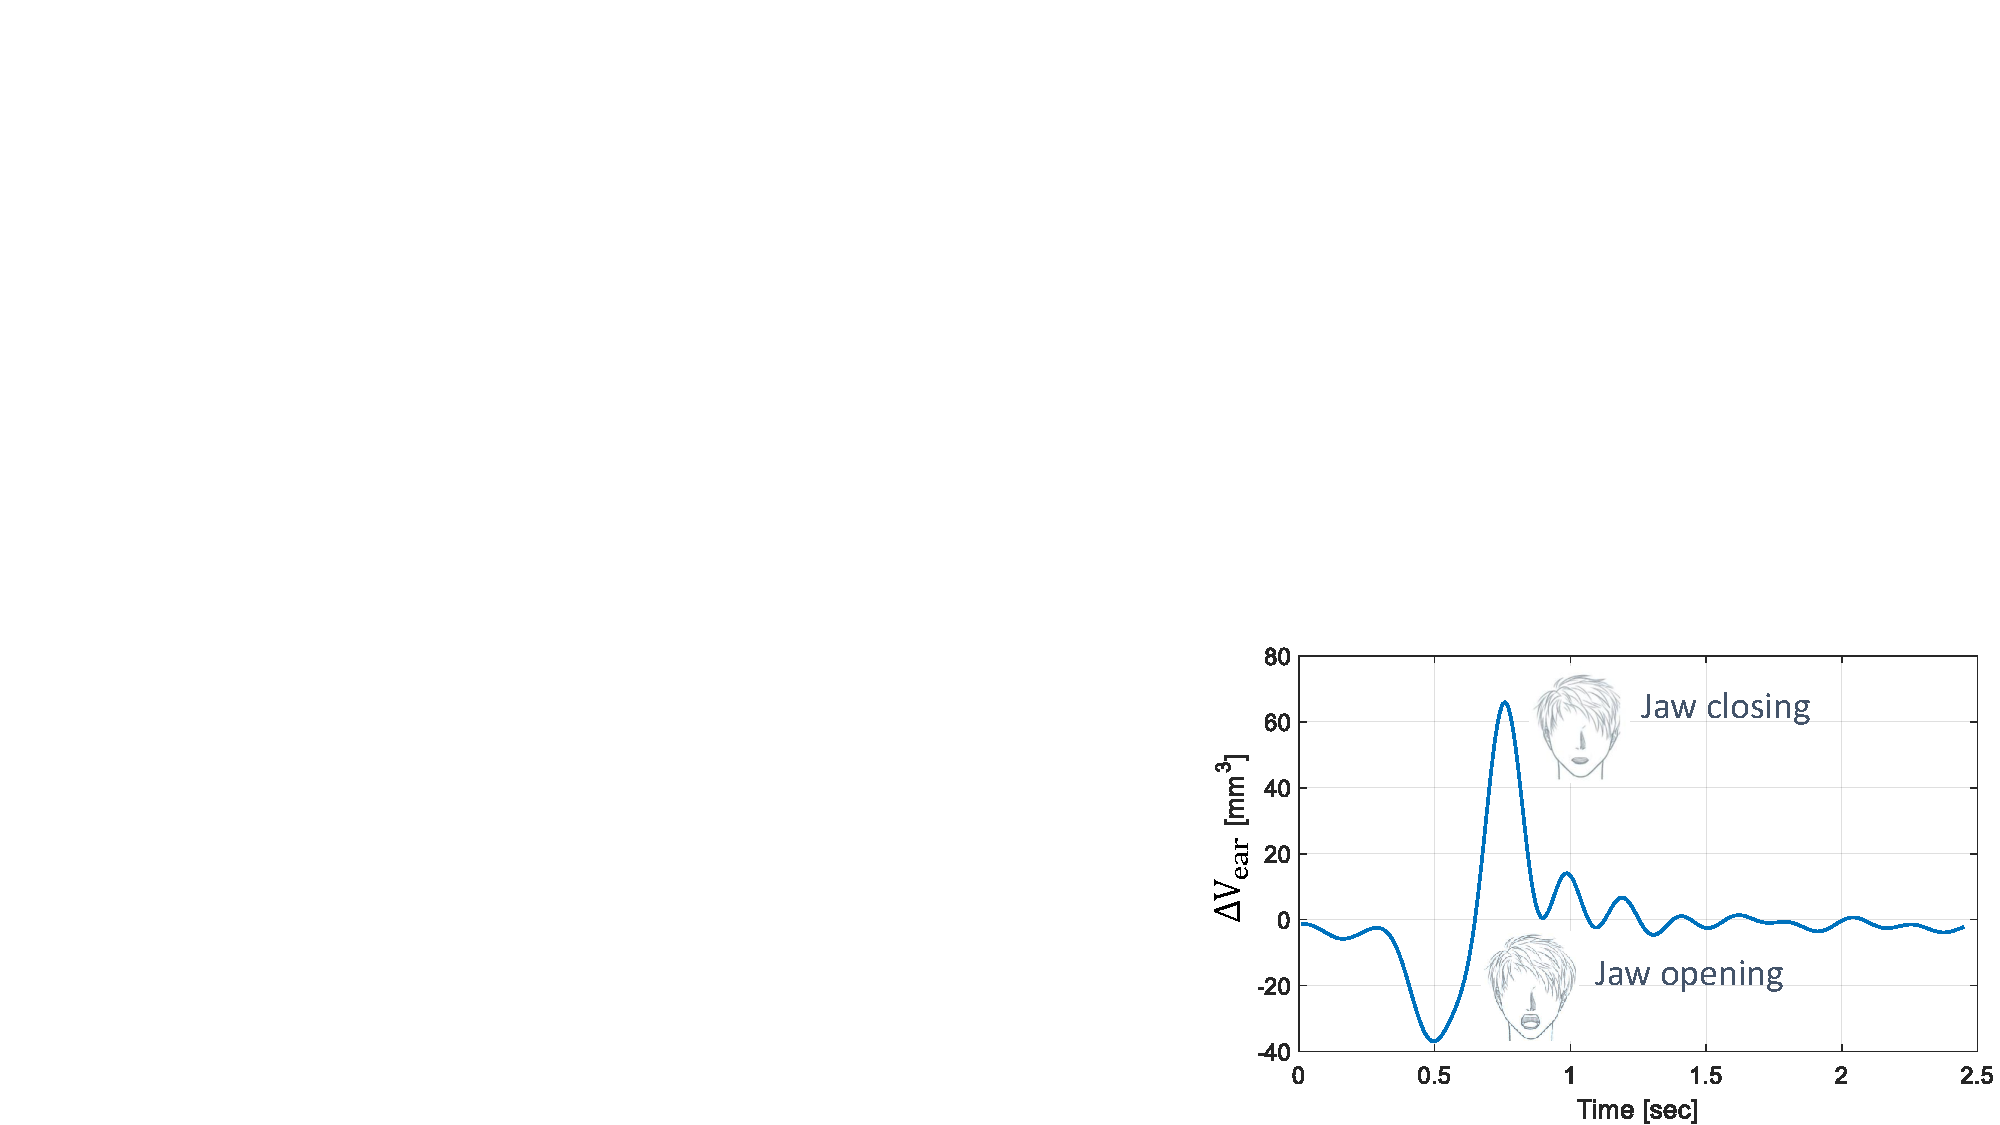
\includegraphics[trim={20.5cm 0cm 0cm 10.8cm},clip, width=0.4\textwidth]{figures/deltaV_ear.pdf}
	\caption{Earcanal volume variation for one mastication cycle}
	\label{fig:deltaV_ear}
\end{figure}
%%%%%%%%%%%%%%%%%%%%%%%%%%%%%%%%%%%%%%

The characteristics of the liquid filled earplug's operating behavior have not been studied yet. Thus, the evolution of the volume variation $\Delta V_{ear}$ is not well known as a function of the pressure variation $\Delta p_{ear}$. Considering the pressure and volume variation levels from \cite{Delnavaz2012} and \cite{Bouchard-Roy2020}, equation \ref{eq:max_hydraulic_energy} approximates an upper limit for the extractable hydraulic energy with the maximum values of $\Delta p_{ear}$ and $\Delta V_{ear}$ that have been recorded, i.e. $p_c=12$\,kPa and $(\Delta V_{ear})_{max}=60$\,mm$^3$. $p_c$ stands for the comfort pressure by assuming that the user feels discomfort if $\Delta p_{ear}>p_c$. The energy estimation presumes that the earplug is a perfect flow rate source, which is a theoretical hypothesis leading to $0.72$\,mJ available from one mastication. If a person masticates 2200 cycles per day, which is the average according to \cite{Goll2011}, there would be $1.6$\,J available per day, per ear. This amount of energy could theoretically enhance the supply some $19$\,\% of the $17$\,J needed for the state of the art of cochlear implants \cite{Kulah2022}. Further research in both domains related to hearing aids and energy harvesting could lead to fully autonomous devices in the future.
\begin{align}
	\text{max}(E_{hyd}) = p_c \cdot (\Delta V_{ear})_{max} = 0.72\text{\,mJ}
	\label{eq:max_hydraulic_energy}
\end{align}

    %///////////////////////////////////////////// 
	\subsection{The harvesting strategy}	
	\label{The harvesting strategy}
    %/////////////////////////////////////////////
Electromagnetic transducers are usually used to harvest energy from kinetic (vibration) energy sources. In fact, the power density of electromagnetic transducers decreases proportionately to the effective volume of the transducing material and the frequency of the energy sources decreases \cite{Priya2017,Kulah2008}. Also, the fabrication and integration of the coil and moving magnet may be a source of difficulty as their gap should be carefully managed to prevent non-linear and unpredicted responses \cite{Caruntu2001}. 

Piezoelectric ceramics appear to be good candidates for small-scale mechanical energy transduction, but their rigid structure limits their use with soft materials, such as human tissues. Mechanical amplifiers, like flextensional structures, can nevertheless be used to adapt the stress/displacement levels between the energy source and the stiff transducing material \cite{Abdelnaby2016}. Also, the best energy conversion efficiency for piezoelectric ceramics is achieved at the transducer's resonance. As the mean mastication frequency is estimated to \mbox{$1.57$\,Hz}, the harvesting system could benefit from a frequency-up conversion stage to increase the frequency of the energy source, which in turn increases the energy conversion efficiency of the transducer \cite{Ashraf2011,Peng2021}. Most of the frequency-up systems with piezoelectric transducers use mechanical stops with piezoelectric ceramic cantilevers to reach high frequencies with a good mechanical coupling \cite{Edwards2013,Gu2011,Lee2007}. However, stoppers dissipate energy. Alternative solutions use mechanical Bistable Resonators (BR) \cite{Vocca2012}. Recent works led to the development and optimization of bistable structures integrating stacked piezoelectric ceramics within flextensional elastic structures \cite{Huguet2017}. They show enhanced performances due to high electromechanical coupling. Theoretically, the electromechanical converter, composed of a BR with piezoelectric ceramics in a flextensional structure offers a higher energy conversion efficiency than low frequency solutions and/or flexible electromechanical transducers \cite{Abdelnaby2016,Peng2021}.

The hydraulic-mechanic interface can be a hydraulic cylinder (HC). It can store the energy in the frequency-up converter by actuating it at the frequency of human mastication. The amount of extractable energy from the hydraulic source will then depend on the EH mechanical behavior. Before being converted into electricity, the energy is in fact stored in a mechanical potential reservoir. During the low frequency actuation, the forces applied on each side of the HC piston are equal. Equation \ref{eq:hydraulic-mechanic_interface} models the hydraulic-mechanic interface with $x_{m}$ and $ S_{hc}$ being respectively the dynamic mass position on the $\vec{x}$ axis and the HC internal section.
%%%%%%%%%%%%%%%%%%%%%%%%%%%%%%%%%%%%%%
\begin{equation}
	\Delta p_{ear}\ S_{hc} = K_{s}\ x_{m}
	\label{eq:hydraulic-mechanic_interface}
\end{equation}
%%%%%%%%%%%%%%%%%%%%%%%%%%%%%%%%%%%%%%
Therefore, the potential energy stored in a linear resonator from the ideal hydraulic source previously described can be expressed as follows:
\begin{equation}
	Ep_{lin} = \dfrac{K_s\ x_{m}^2}{2} = \dfrac{\Delta p_{ear} \Delta V_{ear}}{2}
	\label{eq:best_linear_soution}
\end{equation}
Thus, the linear solution can theoretically exploit/store a maximum of $50\,\%$ from the maximum available hydraulic energy ($\text{max}(E_{hyd})$). 

Non-linear elastic potential reservoirs can also be considered. This work presents the energy extraction capability of a BR governed by a Duffing equation. It admits 2 stable equilibrium positions \mbox{$x_m=\pm x_0$}, an unstable one in \mbox{$x_m=0$} and its stiffness depends on its structural buckling level $\epsilon$ defined later in equation \ref{eq:epsilon_def}. The maximum theoretical energy in the BR for a quasi-static actuation is equal to the height of the potential energy barrier $E_{pb}$ when the mass position varies from \mbox{$x_m=\pm x_0$} to \mbox{$x_m=0$} (Eq. \ref{eq:Ep_bar}). It will be a fraction $n$ of the upper limit of the available hydraulic energy (Eq. \ref{eq:max_hydraulic_energy}), where $n$ has to be maximized. 
\begin{equation}
	E_{pb} = \dfrac{K x_0^2\epsilon^2}{3} = n(p_c \cdot (\Delta V_{ear})_{max})
	\label{eq:Ep_bar}
\end{equation}
Hence, we see that it is inherently capable of exploiting $65$\,\% from the hydraulic energy source, which is $15$\,\% better than the best theoretical linear option. Section \ref{sec:SYSTEM MODELING} will discuss the modeling and design of a non-linear BR harvester, as this appears to be a better solution than the linear approach. 
%/!\/!\/!\/!\/!\/!\/!\/!\/!\/!\/!\/!\/!\/!\/!\/!\/!\/!\/!\/!\/!\/!\/!\/!\%
\section{ENERGY HARVESTER PRESENTATION AND OPERATION \mbox{PRINCIPLE}}
\label{sec:HARVESTER PRESENTATION AND OPERATION PRINCIPLE}
%/!\/!\/!\/!\/!\/!\/!\/!\/!\/!\/!\/!\/!\/!\/!\/!\/!\/!\/!\/!\/!\/!\/!\/!\%
%%%%%%%%%%%%%%%%%%%%%%%%%%%%%%%%%%%%%%%
\begin{figure*}[!htbp]
	\centering
	\captionsetup{justification=centering}
	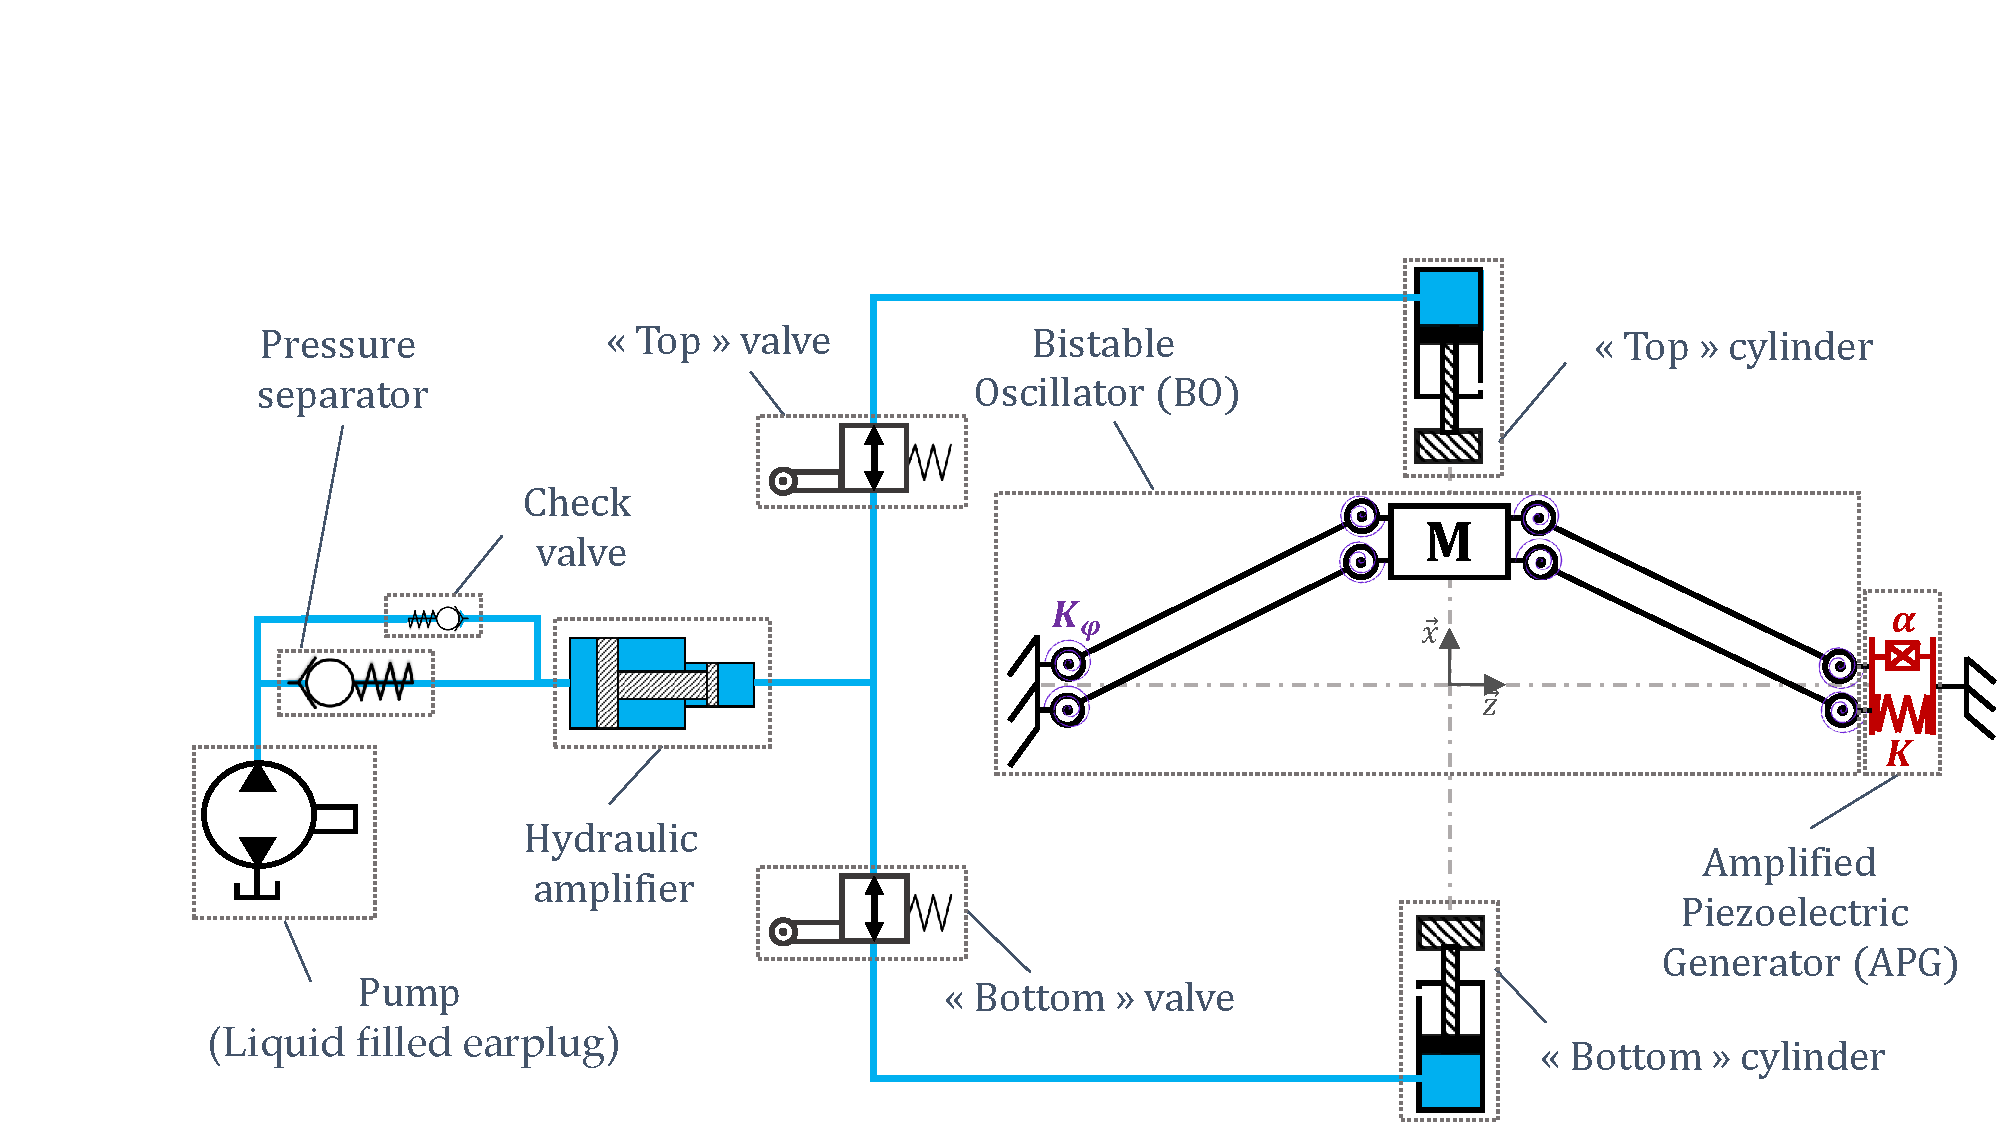
\includegraphics[trim={3.2cm 0cm 0cm 4.3cm},clip, width=0.7\textwidth]{figures/system_presentation.pdf}
	\caption{Schematic presentation of the frequency-up piezoelectric EH exploiting the earcanal's geometry variation} 
	\label{fig:system_presentation}
\end{figure*}
%%%%%%%%%%%%%%%%%%%%%%%%%%%%%%%%%%%%%%%
Figure \ref{fig:system_presentation} is a schematic view of the energy harvesting system. In this system, a liquid-filled earplug transmits the energy beyond the earcanal. To maximize its efficiency, the system is equipped with a BR frequency-up conversion mechanism. The BR is connected to an Amplified Piezoelectric Generator (APG) \cite{CEDRATTECHNOLOGIES2022} made of a flextensional elastic APX4 steel \cite{AUBERT&DUVAL2022} structure that contains stacked lead zirconate titanate (PZT) ceramics (Fig. \ref{fig:APG}).
%%%%%%%%%%%%%%%%%%%%%%%%%%%%%%%%%%%%	
\begin{figure}[!htb]
	\begin{center}
		\begin{subfigure}[t]{0.5\linewidth}
			\captionsetup{justification=centering}
			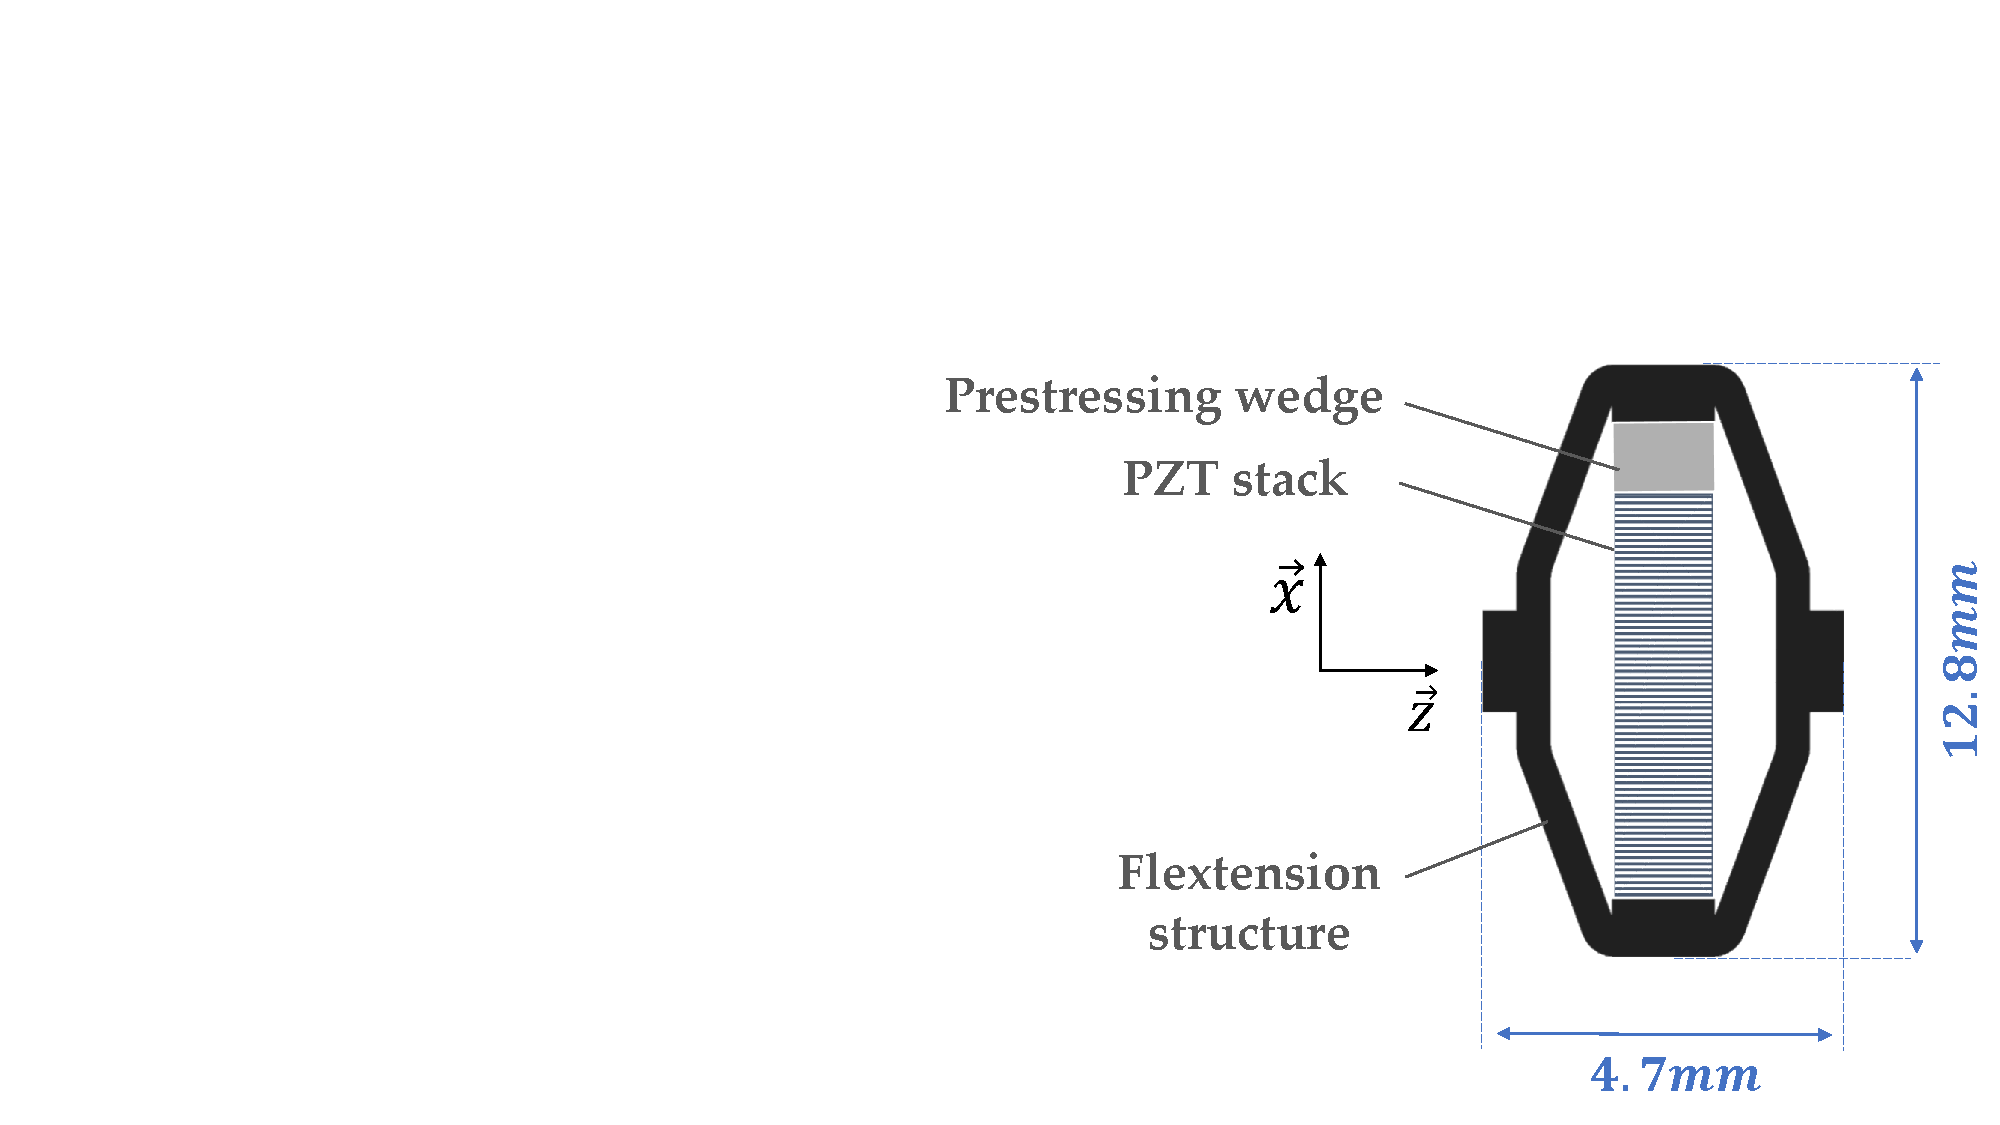
\includegraphics[trim={13cm 0cm 0cm 6cm},clip,width=\linewidth]{figures/APG_schema.pdf}
			\caption{Detailed schema}
			\label{fig:APG_schema}
		\end{subfigure}
		\hfillx
		\begin{subfigure}[t]{0.21\linewidth}
			\captionsetup{justification=centering}
			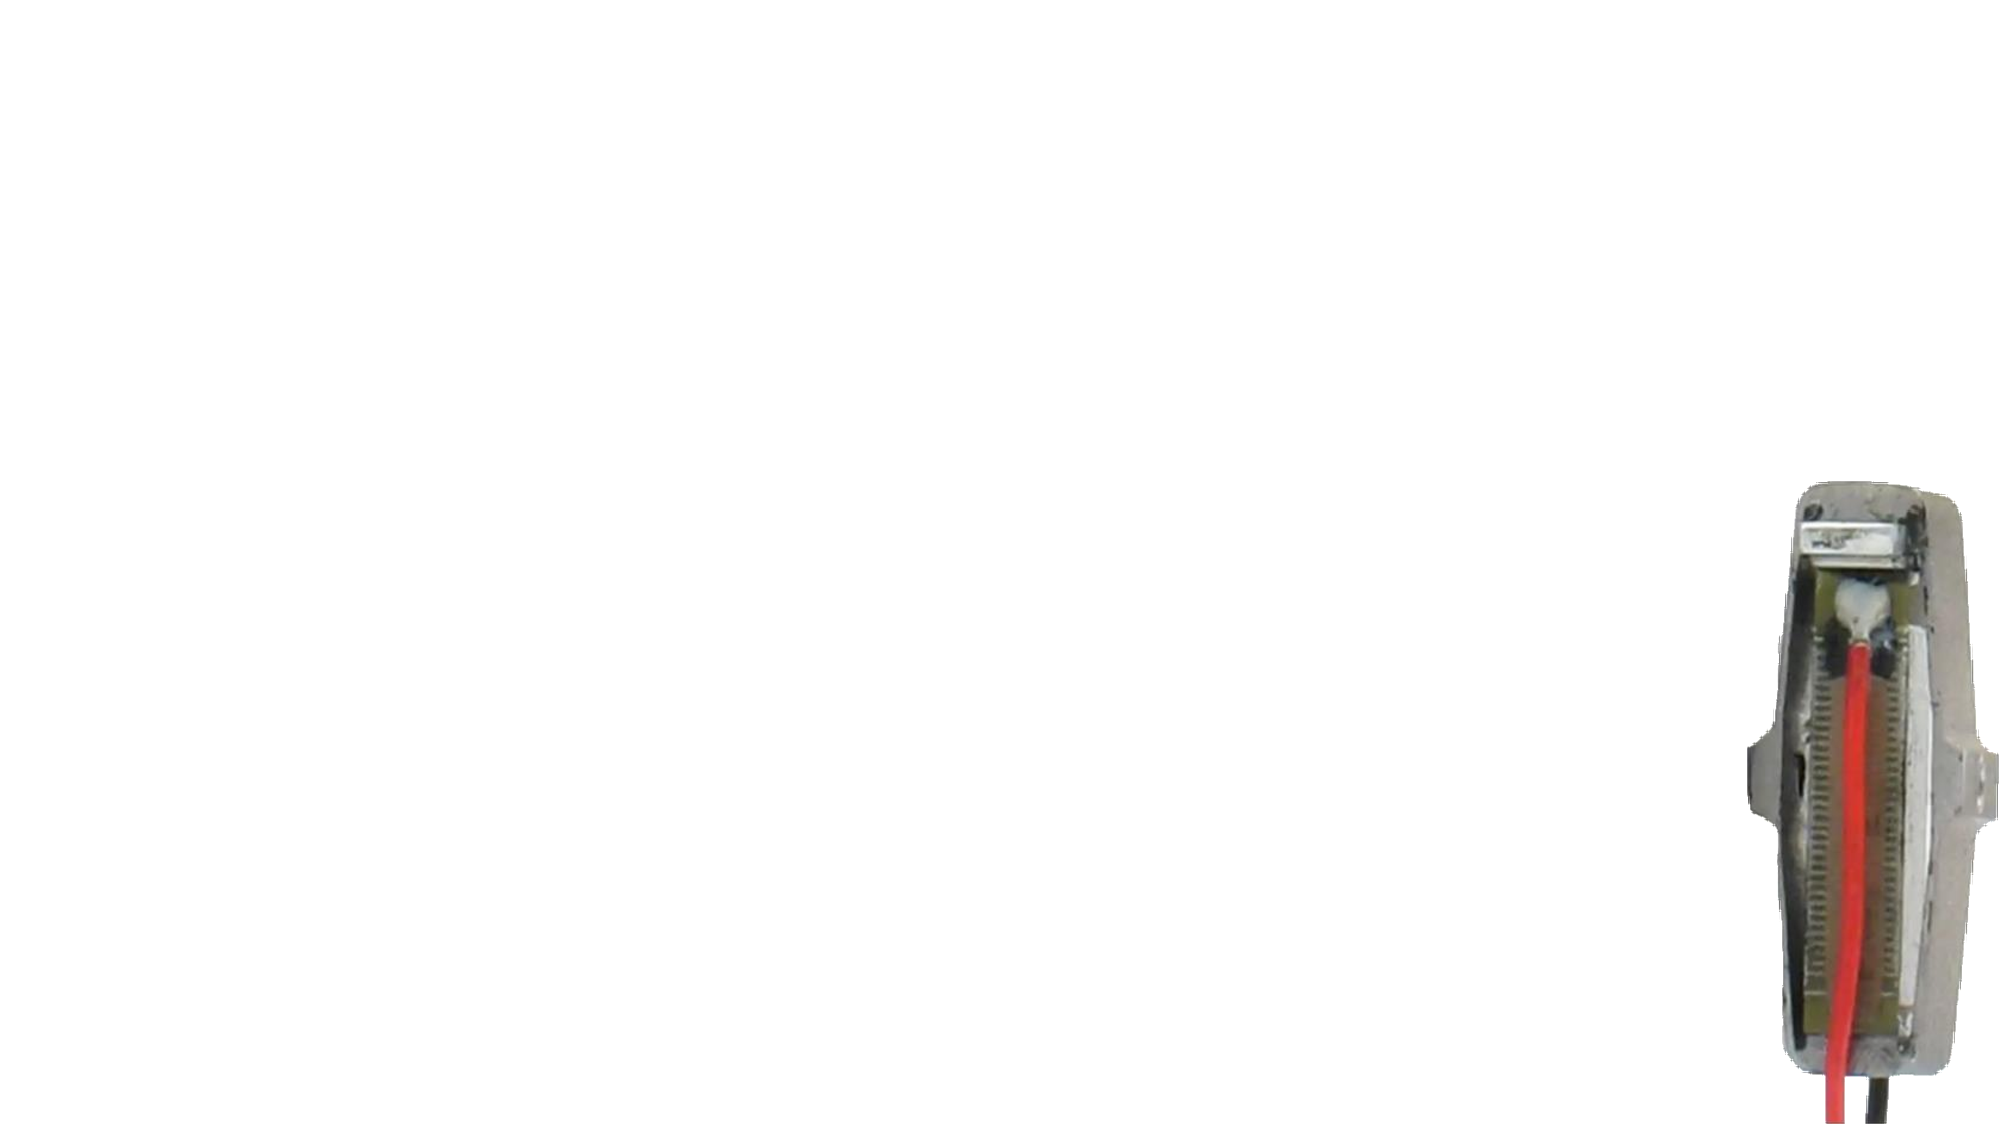
\includegraphics[trim={29.5cm 0cm 0cm 8cm},clip,width=0.65\linewidth]{figures/APG_photo.pdf}
			\caption{Picture}
			\label{fig:APG_photo}
		\end{subfigure}
		\caption{Amplified Piezoelectric Generator (APG)}
		\label{fig:APG}
	\end{center}
\end{figure}
%%%%%%%%%%%%%%%%%%%%%%%%%%%%%%%%%%%% 

The APG is actuated by two hydraulic cylinders (HC) using the hydraulic energy transmitted from the liquid-filled earplug trough a hydraulic amplifier (HA) and two hydraulic valves (HVs). During a mastication cycle, the TMJ compresses the earcanal wall which expels the fluid out of the earplug. The HVs lead the fluid alternatively to each HC to actuate the BR mass back and forth. The HA can simultaneously adapt the cylinders' stroke to the available earplug swept volume, and the actuation force of the BR to the comfort pressure of the earcanal (Fig. \ref{fig:system_presentation}).

The BR mass has two equilibrium positions, \mbox{$x_m = x_0$ } and \mbox{$-x_0$}. The EH operates during two major phases. The first is when the BR mass is actuated by the HC, from one equilibrium position toward the unstable position at $x_m = 0$. During the second phase the mass reaches and oscillates around the opposite equilibrium position until it stops, while a portion of the vibration energy is converted into electricity by the APG. The mass will move backward when the next mastication action occurs and this completes one energy harvesting cycle.
%%%%%%%%%%%%%%%%%%%%%%%%%%%%%%%%%%%%%%%
\begin{figure}[!htbp]
	\centering
	\captionsetup{justification=centering}
	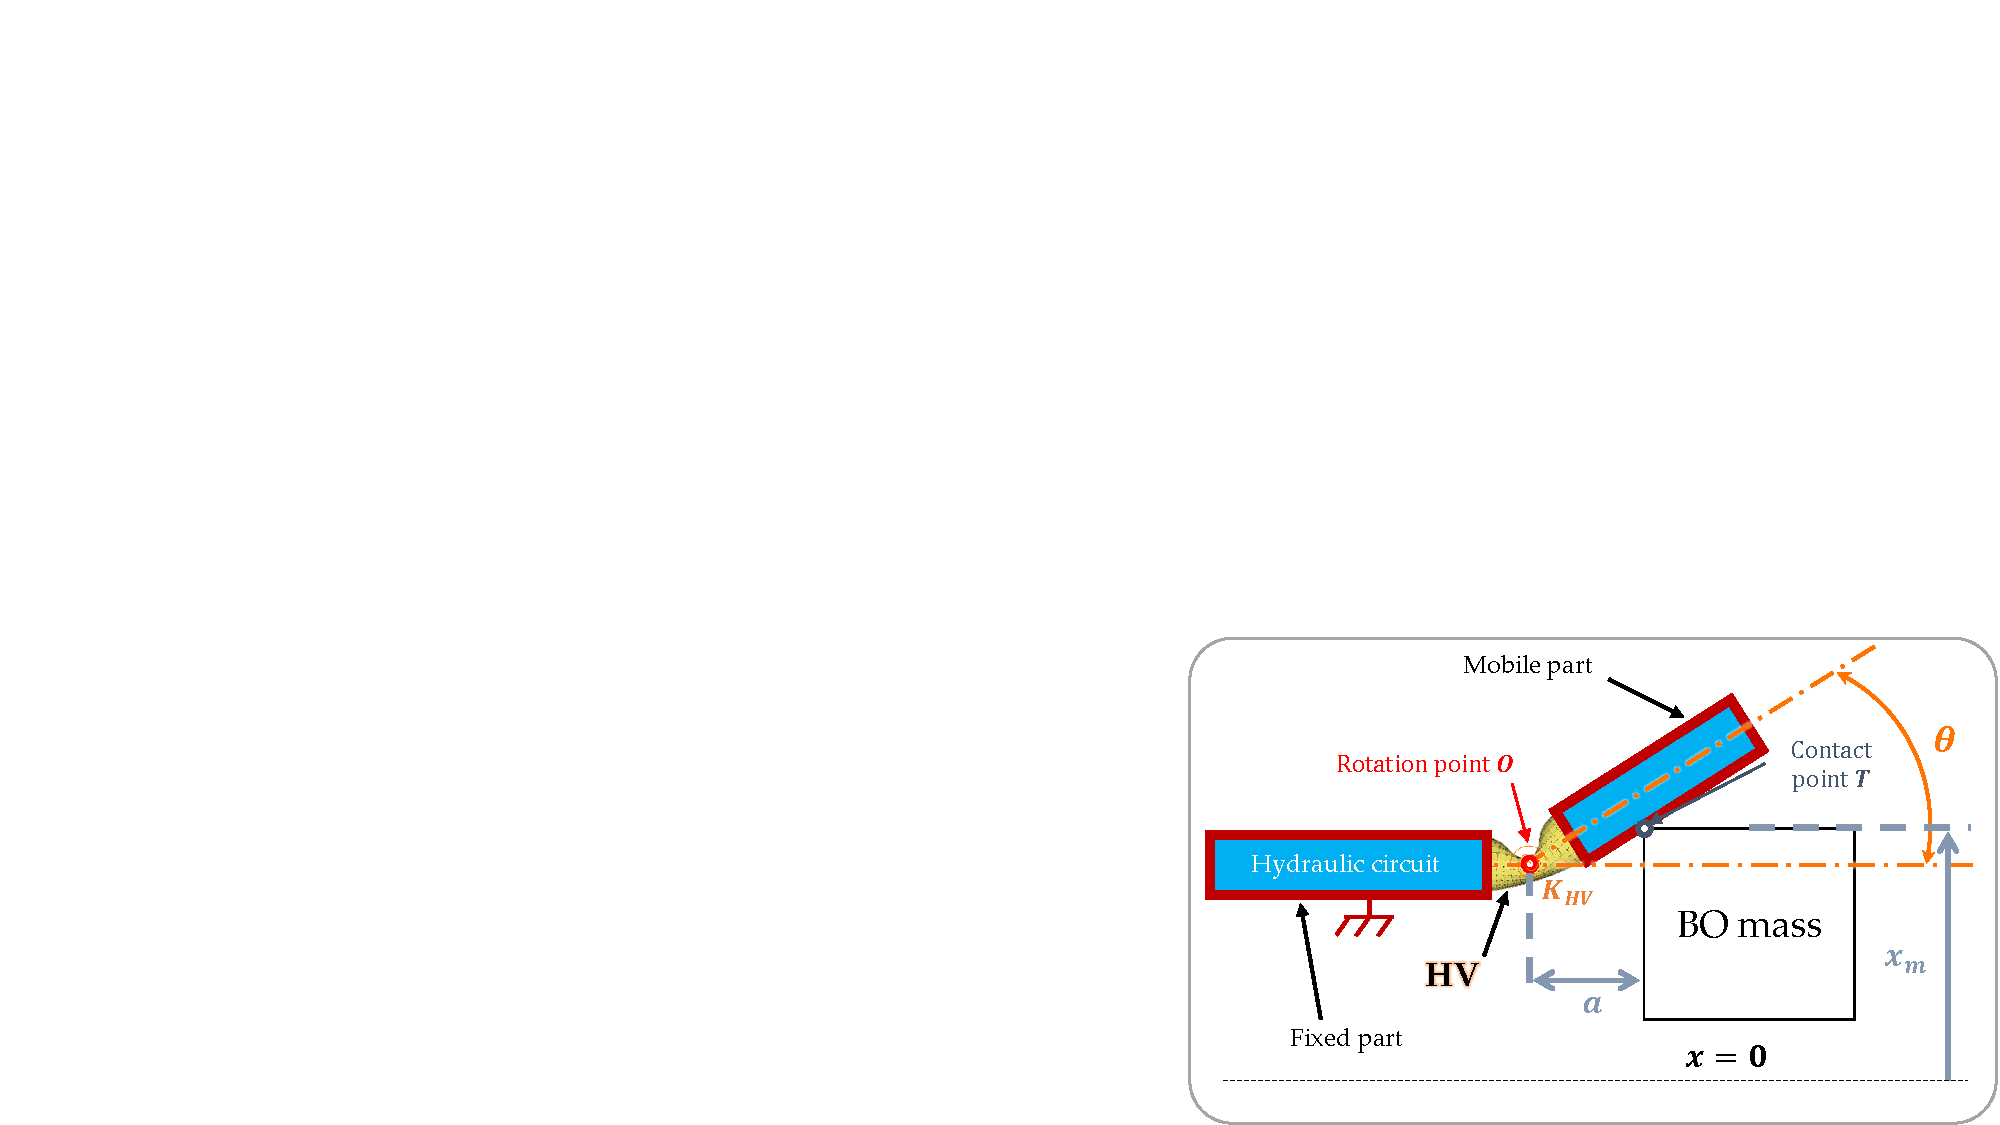
\includegraphics[trim={20.5cm 0cm 0cm 11.5cm},clip, width=0.8\linewidth]{figures/HV_actuation_detail.pdf}
	\caption{Details of the contact between a HV and the BR mass} 
	\label{fig:HV_actuation_detail}
\end{figure}
%%%%%%%%%%%%%%%%%%%%%%%%%%%%%%%%%%%%%%%

A technological solution for the HV is to use a flexible tube buckled by bending. Figure \ref{fig:HV_actuation_detail} illustrates such a HV integrated on the BR. The HV is made of a flexible tube connected to the hydraulic circuit by rigid mobile and rigid fixed sheaths. The HV is in contact with the mass at point T. The mass motion on the mobile sheath induces a bending angle $\theta$ around rotational point $O$ located at the buckled section of the flexible tube. Consequently, a pressure loss is generated through the valve in its buckled position. The HV is to be closed when the BR mass is at a stable equilibrium position ($x_m=\pm x_0$) and to be opened when the mass is at $x_m=0$. This sequence of the valve opening and closing will be investigated experimentally in section \ref{sec:EXPERIMENTAL APPROACH FOR THE HV DESIGN}. Two HVs symmetrically placed on either side of the $\vec{z}$ axis set up an open hydraulic circuit on one side and a closed one on the other, depending on the BR mass's position. This technological choice for the HV is motivated by three main arguments. First, the absence of dedicated electromechanical transduction compared to the more commonly used actuated valve minimizes the energy losses during the valve's operation. Second, the post-buckling softening effect of the bent tube minimizes the mechanical impact on the BR mass dynamic operation. Finally, it seems to be well adapted for applications on millimetric scales.
%/!\/!\/!\/!\/!\/!\/!\/!\/!\/!\/!\/!\/!\/!\/!\/!\/!\/!\/!\/!\/!\/!\/!\/!\%
\section{SYSTEM GLOBAL MODELLING}
\label{sec:SYSTEM MODELING}
%/!\/!\/!\/!\/!\/!\/!\/!\/!\/!\/!\/!\/!\/!\/!\/!\/!\/!\/!\/!\/!\/!\/!\/!\%
The EH is a multiphysics system composed of hydraulic, mechanical, and electrical components. This section presents the global multiphysics model and describes the system's theoretical basis of operation. Two coupled subsystems are considered. Subsection \ref{subsec:The electromechanical converter} shows the modelling of the electromechanical frequency-up converter (BR + APG) under the mechanical influence of the HV and HC. Subsection \ref{subsec:The hydraulic circuit} discusses the design of the hydraulic circuit composed of the two HVs, two HCs, HA and liquid-filled earplug.

The challenge of this work lies in the experimental validation of the electromechanical converter cycled by two HVs and two HCs. Several hydraulic miniature solutions for HAs and HCs have already been presented in the literature \cite{Wang2020,Xu2021,Zhu2013}. The energy loss associated with these components has been neglected in this paper and will be considered in our further works. 
    %///////////////////////////////////////////// 
	\subsection{Modelling of the electromechanical converter}	
	\label{subsec:The electromechanical converter}
    %/////////////////////////////////////////////
%%%%%%%%%%%%%%%%%%%%%%%%%%%%%%%%%%%%%%
\begin{figure*}[!htbp]
	\centering
	\captionsetup{justification=centering}
	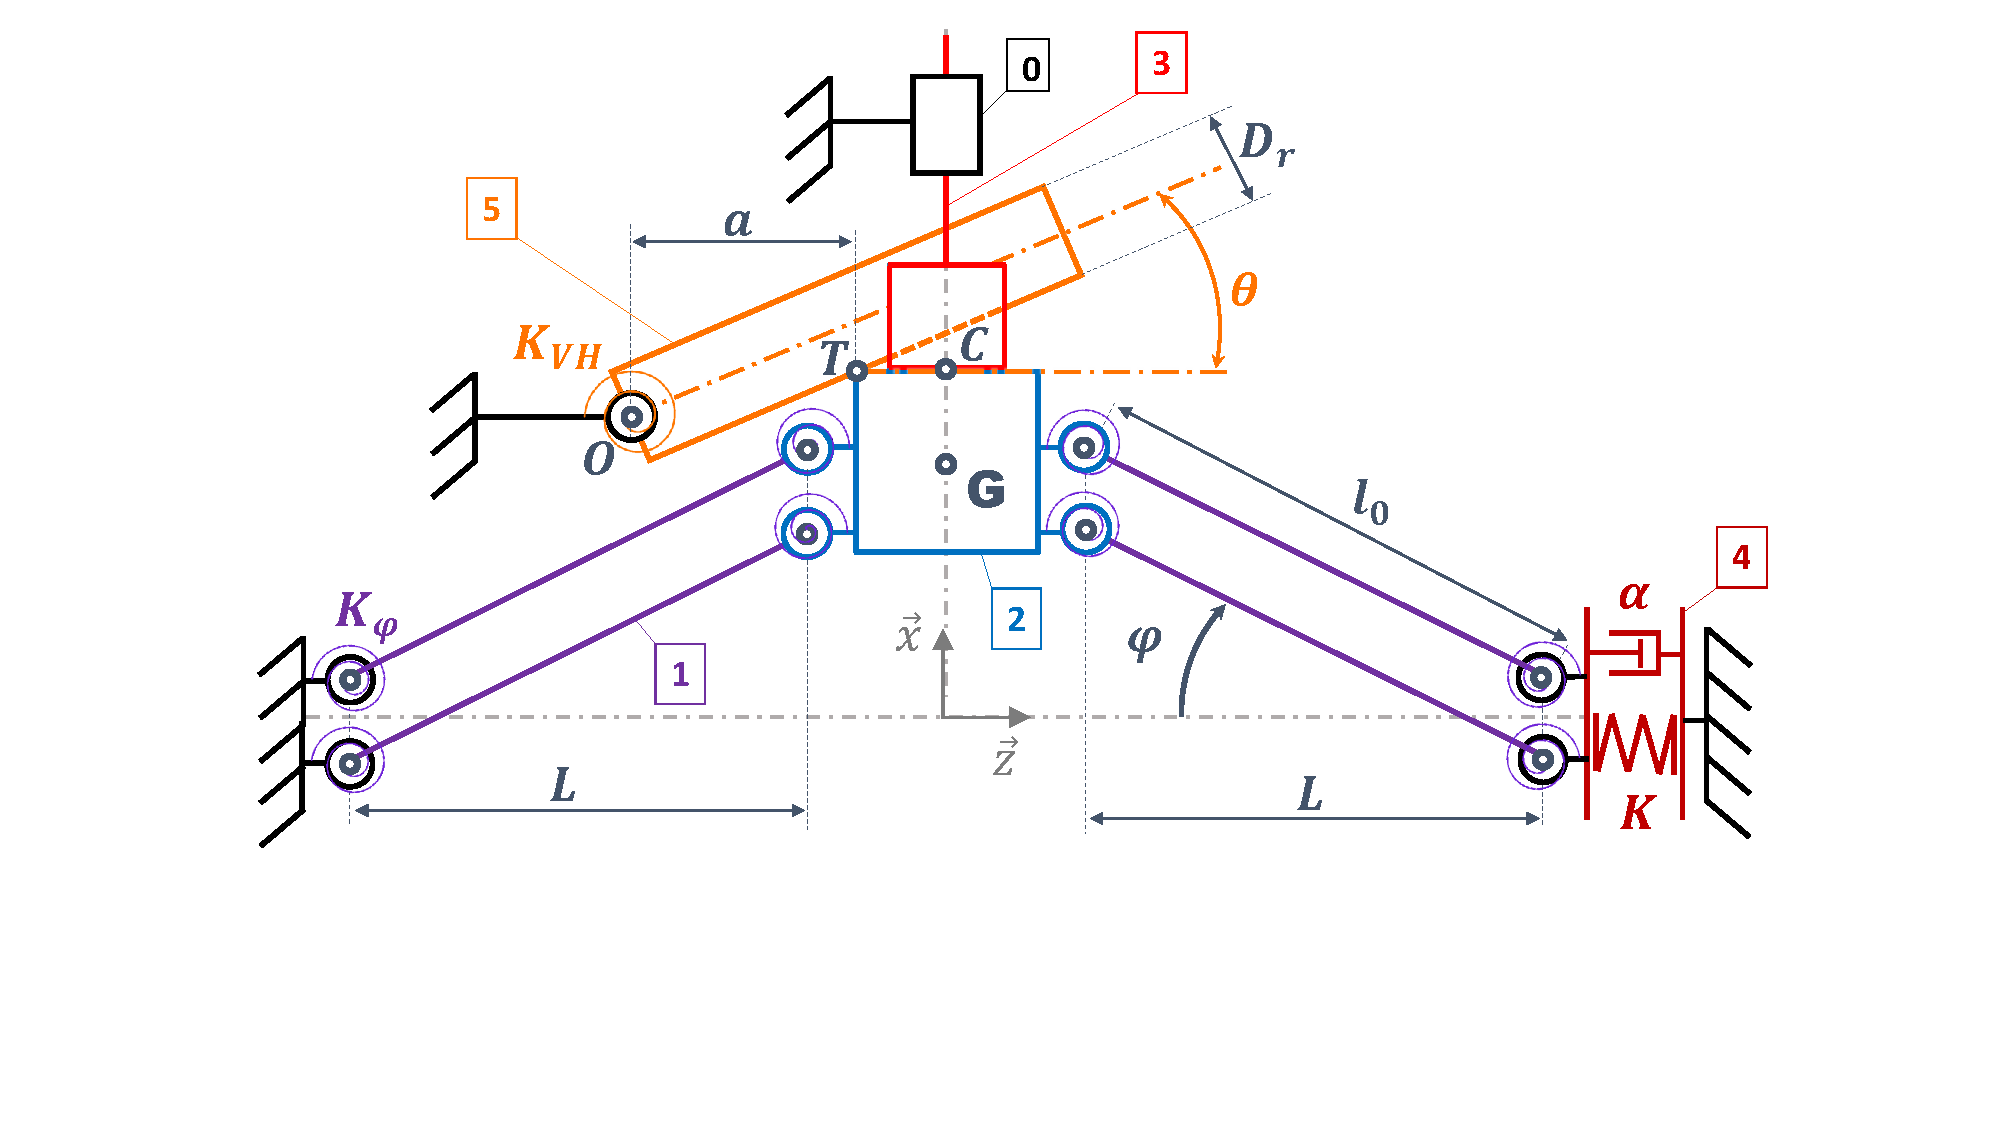
\includegraphics[trim={0cm 0cm 0cm 0cm},clip, width=0.9\textwidth]{figures/schema_cinematique1.pdf}
	\caption{Kinematic scheme of the electromechanical converter under the mechanical influence of a HV and HC}
	\label{fig:schema_cinematique1}
\end{figure*}
%%%%%%%%%%%%%%%%%%%%%%%%%%%%%%%%%%%%%%

Figure \ref{fig:schema_cinematique1} shows the kinematic scheme of the electromechanical converter under the mechanical forces of the HV and HC. The various rigid bodies are defined in Table \ref{tab:Designation of rigid bodies}. The BR is shown as 4 identical arms articulated by 8 hinges and a central mass. The hinge's angle $\varphi$ is defined by:
\begin{equation}
	\varphi = \arctan\biggl(\dfrac{x_m}{L}\biggr)
	\label{eq:phi_definition}
\end{equation}
The APG is considered as a spring of stiffness $K$ with an electromechanical coupling $k^2$, standing for the piezoelectric transduction and defined by Equation \ref{eq:k2_def}.\\
\begin{equation}
	k^2 = \dfrac{\alpha^2}{\alpha^2 +  K C_p}
	\label{eq:k2_def}
\end{equation}
The model is based on the following hypotheses:
\begin{itemize}
	\item The only mass considered is the BR mass (2).
	\item All parts are rigid except for the APG (4).
	\item The hinges are considered elastic: They are defined by their rotational stiffness $K_{\varphi}$
	\item The mechanical damping of the hinges is included in the global viscous damping coefficient $\mu$.
	\item The contact between the BR mass (2) and the HC piston head (5) is considered permanent for $0 < x < x_0$.
	\item \mbox{$x_0 \ll L$}. 
\end{itemize}

%%%%%%%%%%%%%%%%%
\begin{table}[!htbp]
\centering
\resizebox{0.6\linewidth}{!}{%
	\begin{tabular}{ c | c }
		\toprule
		\multicolumn{1}{c}{\textbf{Num}} &
		\multicolumn{1}{c}{\textbf{Name}}                                 \\
		\midrule
		0                                & Fixed frame                    \\
		1                                & BR arm                         \\
		2                                & BR mass                        \\
		3                                & HC piston head                 \\
		4                                & APG                            \\
		5                                & Simplified HV mechanical model \\
		\bottomrule
	\end{tabular}}
\caption{Definition of figure \ref{fig:schema_cinematique1} bodies}
\label{tab:Designation of rigid bodies}
\end{table}
%%%%%%%%%%%%%%%%%%%%%  

By isolating the BR mass and using Newton's 2$^{nd}$ law, we can express its dynamic equilibrium. The projection on the $\vec{x}$ axis of the resulting expression is given by Equation \ref{eq:OB-GPA}. The BR mechanical equilibrium has a mass inertial term, a non-linear stiffness depending on $x_m$, the stiffness of the hinge $K_{\varphi}$ and viscous losses. The first term introduced by the HV is related to its rotational stiffness $K_{HV}$ and the second term is related to the friction losses at contact point $T$ (see fig. \ref{fig:HV_actuation_detail}). $K_{HV}$ and $K_{\varphi}$ both act in the same way by shifting the stable equilibrium positions of the BR toward $0$ as much as they increase. A dry friction model is chosen to describe the dissipation effect of the contact. The rubbing efforts depend on a dry friction coefficient $f_d$, related to the nature of the materials that are rubbing together, and by the sign of $\dot{x}_m$. Pressure $p_{hc,a}$ induces the HC hydraulic force, and coefficient $\mu_{hc}$ models the viscous friction at the sealing gasket of the HCs. The hydro-mechanical coupling will be detailed later.

The electrical power generated by the APG is dissipated in a load resistor $R_l$, calculated using adaptive impedance matching, as expressed in Equation \ref{eq:R_ch_adaptive_imp} \cite{Liu2013}. 
\begin{equation}
	R_l = \dfrac{1}{C_p w_0}
	\label{eq:R_ch_adaptive_imp}
\end{equation}
Thus, the electrical equation of the APG is:
\begin{equation}
	\dfrac{U_p}{R_l} = 
	-\alpha\dfrac{d}{dt}\biggl(2\sqrt{{l_0}^2-x_m^2}\biggr)
	- C_p\dot{U}_p
	= \frac{2\alpha x_m\dot{x}_m}{\sqrt{L^2+x_m^2}} - C_p\dot{U}_p
\label{eq:APG_elec}
\end{equation}
Consequently, the generated power $P_e$ expression is:
\begin{equation}
	P_e = \frac{{U_p}^2}{R_l} 
	\label{eq:P_e}
\end{equation} 
Equation \ref{eq:theta_fonction_de_xm} defines the implicit relation between $\theta$, $x_m$ and the geometrical parameters of the setup. Additionally, the HV stiffness $K_{HV}$ will depend on its bending angle $\theta$, as showed in Figure \ref{fig:HV_actuation_detail}.  
%%%%%%%%%%%%%%%%%%%%%%%
\begin{figure*}[!htb]
\begin{equation}
 m \ddot{x}_m =-2K_{eq}(\sqrt{x_m^2+L^2}-l_0)\tan(\varphi(x_m)) -\mu \dot{x}_m -\frac{4K_{\varphi}\varphi}{L}
				\ -2\alpha U_p \tan(\varphi(x_m))
				\ -\dfrac{K_{HV}(x_m)\theta(x_m)}{a}\biggl(1 - f_d \text{sign}(\dot{x}_m)\biggr)
				\  - p_{hc,a}\ S_{hc} - \mu_{c}\ \dot{x}_m
\label{eq:OB-GPA}
\end{equation}
\end{figure*}
% \FloatBarrier
%%%%%%%%%%%%%%%%%%%%%%%
%%%%%%%%%%%%%%%%%%%%%%%
\begin{equation}
\resizebox{.9\linewidth}{!}{$	
x_m = \Biggl[ \dfrac{D_r(1-\cos(\theta))+2a\sin(\theta)}{2\cos(\theta)}\text{,}
				~~ \theta\leq\arctan\biggl(\dfrac{2a}{D_r}\biggr) \Biggr]
				$}
\label{eq:theta_fonction_de_xm}
\end{equation}

%%%%%%%%%%%%%%%%%%%%%%%
    %///////////////////////////////////////////// 
	\subsection{Modelling of the hydraulic circuit}	
	\label{subsec:The hydraulic circuit}
    %/////////////////////////////////////////////
In order to model the coupled behavior of the two hydraulic branches, we will use the index "$a$" for the active branch where the fluid flows and the index "$i$" for the inactive one. \\
The following hypotheses will be considered:
\begin{itemize}
	\item The flow is incompressible and Newtonian.
	\item The hydraulic circuit is rigid (no volume change) and there is no leakage.
	\item The hydraulic actuation is considered quasi-static considering the oscillation frequency of the BR.
\end{itemize}
The mechanical equilibrium is:
\begin{align}
	\text{Inactive cylinder ~}& \left\{~
	p_{hc,i}\ S_{hc} - \mu_{c}\ \dot{x}_{hc,i} = 0
	\right.
	\label{eq:equilibre_dynamique_piston_ferme}
\end{align}
The pressure loss coefficient $Cf$ for a buckled flexible tube will depend on the HV bending angle $\theta$ and on the BR mass's position $x_m$ (Fig. \ref{fig:HV_actuation_detail}). $Cf$ will be all the more important as $x_m$ increases. Its minimal value $Cf_0$ is obtained when the HV is unbent. We assume at first that the relationship between $Cf$ and $x_m$ is linear and defined as follows:
\begin{align}
Cf(x_m) & = Cf_0 + \dfrac{Cf_c - Cf_0}{x_0}\ |x_m| 
\label{eq:Cf(x_m)_linear}
\end{align}
where $Cf_c=Cf(\pm x_0)$. Regarding the BR symmetry, the relation between $Cf$ and $x_m$ must be an even function to enable the system cycling, i.e., $Cf(x_m) = Cf(-x_m)$.

Using Bernoulli's equation for a current line, we can express the earplug's internal pressure $p_{ear}$ as a function of the hydraulic resistance in the two parallel branches with Equations \ref{eq:Bernoulli_piston_ouvert} and \ref{eq:Bernoulli_piston_ferme}.
\begin{align}
	\text{Active branch ~}& \left\{~
	p_{ear} = \dfrac{1}{a_h}\biggl(p_{hc,a} + Cf_0 {q_a}^2 \biggr)
	\right.
	\label{eq:Bernoulli_piston_ouvert}\\
	\text{Inactive branch ~}& \left\{~
	p_{ear} = \dfrac{1}{a_h}\biggl(p_{hc,i} + Cf(x_m) {q_i}^2 \biggr)
	\right.
	\label{eq:Bernoulli_piston_ferme}
\end{align}
where $a_h$ is the hydraulic amplification ratio and $q$ the fluid flow rate.

The no-leakage assumption means that any fluid exciting the earplug flows into the two hydraulic branches (Eq. \ref{eq:conservation_masse}).
\begin{equation}
	q_{ear} = \dot{\Delta V_{ear}} = q_a + q_i
	\label{eq:conservation_masse}
\end{equation}
Moreover, the fluid entering the HC necessarily results in a piston displacement (Eqs. \ref{eq:conservation_masse_ouvert},\ref{eq:conservation_masse_ferme}).
\begin{align}
	\text{Active cylinder ~}& \left\{~
	q_a = S_{hc} \dot{x}_m
	\right.
	\label{eq:conservation_masse_ouvert}\\
	\text{Inactive cylinder ~}& \left\{~
	q_i = S_{hc} \dot{x}_{ic}
	\right.
	\label{eq:conservation_masse_ferme}
\end{align}
%/!\/!\/!\/!\/!\/!\/!\/!\/!\/!\/!\/!\/!\/!\/!\/!\/!\/!\/!\/!\/!\/!\/!\/!\%
\section{NUMERICAL MODEL AND SIMULATIONS}
\label{sec:NUMERICAL MODEL AND SIMULATIONS}
%/!\/!\/!\/!\/!\/!\/!\/!\/!\/!\/!\/!\/!\/!\/!\/!\/!\/!\/!\/!\/!\/!\/!\/!\%
    %///////////////////////////////////////////// 
	\subsection{Setting the EH parameters}	
	\label{subsec:The harvester setting}
    %/////////////////////////////////////////////
The energy system combines several variable parameters. To determine these, we first need to identify the fixed technological elements: 
\begin{itemize}
	\item The transducer is a APA50XS piezoelectric actuator (Cedrat Technologies, Meylan, France) exploited as a generator \cite{CEDRATTECHNOLOGIES2022}.
	\item The hydraulic actuation is ensured by the SMC MQP4-10S HCs which can operate at $1$\,kPa pressure \cite{SMC2022}.
	\item The usual size of a hearing aid case is $50$x$20$x$10$\,mm \cite{Quattro2019}. The \mbox{$L=16$\,mm} parameter is chosen to be consistent with this scale.
\end{itemize}
The system was designed by first setting the two coupled requirements so as to enable the system to work. First, the available swept volume must produce a large enough HC stroke from its equilibrium position until the BR mass reaches \mbox{$x_m=0$} (Eq. \ref{eq:contrainte_course}). The BR mechanical force on the $\vec{x}$ axis reaches a maximum value $F_c$ when \mbox{$ x_m = x_c = \dfrac{x_0}{\sqrt{3}}$}. At this point, a maximum pressure is induced in the earplug and Equation \ref{eq:contrainte_confort} needs to be verified to remain within the pressure limit. If it exceeds the limit, $\epsilon$ can be decreased, diminishing the extracted energy.
\begin{empheq}[left=\empheqlbrace]{align} 
	(\Delta V_{ear})_{max} = a_h\ S_{hc}\  x_{c0}
	\label{eq:contrainte_course}\\
	p_c > \frac{1}{a_h} \frac{F_c}{S_{hc}} ~~~~ \text{with} ~~~~ 
	        F_c = \dfrac{4Kx_0\epsilon}{3\sqrt{3}}
	\label{eq:contrainte_confort}
\end{empheq}
\begin{equation}
	\epsilon = \dfrac{x_0}{L}
	\label{eq:epsilon_def}
\end{equation}
Equations \ref{eq:contrainte_course} and \ref{eq:contrainte_confort} set the amplification level $a_h$ and the BR buckling level $\epsilon$. Regarding the technological choices and the system operation requirements, we can evaluate $n=65\%$ (Eq. \ref{eq:Ep_bar}). This value can be compared to the best theoretical linear energy extraction solution described in Section \ref{eq:best_linear_soution}.
	%///////////////////////////////////////////// 
	\subsection{Targeted hydraulic behavior of the HVs}	
	\label{subsec:HV hydraulic targeted behaviour}
	%/////////////////////////////////////////////
A multiphysics coupled model has been established with the equations and the preliminary dimensioning previously introduced. The key parameter that remains unknown is the hydraulic behavior $Cf(x_m)$ of the HVs. The ratio between the pressure loss coefficient of the closed HV and that of the opened HV must be sufficient to force the flow through the opened branch. Thus, we introduced a hydraulic restriction coefficient $r_{Cf}$, defined as follows:
\begin{equation}
	r_{Cf} = \dfrac{Cf(\text{Closed HV})}{Cf(\text{Opened HV})}	= \dfrac{Cf_c}{Cf_0}	
	\label{eq:r_Cf_definition}
\end{equation}
The numerical resolution of the coupled differential equations \ref{eq:APG_elec},\ref{eq:OB-GPA}, \ref{eq:equilibre_dynamique_piston_ferme}, \ref{eq:Bernoulli_piston_ouvert}, \ref{eq:Bernoulli_piston_ferme}, \ref{eq:conservation_masse}, \ref{eq:conservation_masse_ouvert} and \ref{eq:conservation_masse_ferme} can provide the minimum value $(r_{Cf})_{min}$ that needs to be reached to achieve an adequate hydraulic commutation.
	%///////////////////////////////////////////// 
	\subsection{Simulation results}	
	\label{subsec:Simulation results}
	%/////////////////////////////////////////////
By imposing a volume variation of $\Delta V_{ear}(t)$ recorded during the mastication cycle of a human subject (Fig. \ref{fig:deltaV_ear}), the numerical model gives the theoretical temporal evolution of the hydraulic, mechanical and electrical coupled variables defining the EH. The earplug is assumed to be a perfect flow rate source. The mastication cycle is identically applied 4 times to test the system's cycling robustness. The fixed, designed and resulting theoretical parameters of the simulated global model are presented in Tables \ref{tab:parametres électromécaniques} and \ref{tab:parametres_hydrauliques}.

Figure \ref{fig:positions+DeltaV_debits_pear} shows the simulation results of the mass and HC piston positions overlaid with $\Delta V_{ear}(t)$, the flow rates in the two parallel branches and the earplug pressure. The two different sides are identified on the curves by indexes $t$ for \emph{"top"} side ($x>0$) and $b$ for \emph{"bottom"} side ($x<0$), noting that the effects of gravity are not considered. The same figure shows a focused view on the two main phases of the EH operation during the actuation of the \emph{"bottom"} HC. The simulation begins by the mastication cycle with the following initial conditions:
\begin{itemize}
	\item The mass is at the \emph{"bottom"} equilibrium position $-x_0$.
	\item The \emph{"top"} HV is closed ($Cf_{top} = Cf_c$) and the \emph{"bottom"} side HV is opened ($Cf_{bot} = Cf_0$).
	\item There is no contact between the mass and the HCs.
\end{itemize}

During a first phase, the BR mass is pushed until it reaches $x=0$. The fluid exiting the earplug is mostly guided toward the \emph{"bottom"} HC and a pressure is induced in the earplug by the BR counter-reaction force. The mass then crosses $x_m=0$ and the second phase begins. The \emph{"top"} HV then opens ($Cf_{top} = Cf_0$) and the \emph{"bottom"} side HV closes ($Cf_{bot} = Cf(x_m)>Cf_0$). The fluid is then directed toward the \emph{"top"} side and there is no contact between the mass and an HC. The mass oscillates around $x_m=x_0$ and energy is harvested by the APG. The adequate hydraulic actuation making the fluid flow toward the right HC is achievable when \mbox{$(r_{Cf})_{min}=26$}.  

Figure \ref{fig:positions_Up_puissances_energies} also presents the different positions of the moving components, the APG voltage, the source and harvested powers and the different energies entering and exciting the system. The theoretical global efficiency of the EH is evaluated at \mbox{$\eta_g=85$\,\%} with 22\,µJ electrical energy harvested from one mastication. The energy losses are mostly located in the BR stage and depend on quality factor $Q$ that has been set in accordance with previous work results on similar BR architectures \cite{Liu2013}. The energy source depends on comfort pressure level $p_c$ that is set to 1\,kPa, i.e., a fraction of the theoretical maximal value of $12$\,kPa \cite{Bouchard-Roy2020}. The EH's theoretical efficiency could reach a maximum extractable energy of 398\,µJ from one mastication cycle (Eq. \ref{eq:Ep_bar}).

%%%%%%%%%%%%%%%%%%%%%%%%%%%%%%%%%%%%%%
\begin{figure*}[!htbp]
	\centering
	\captionsetup{justification=centering}
	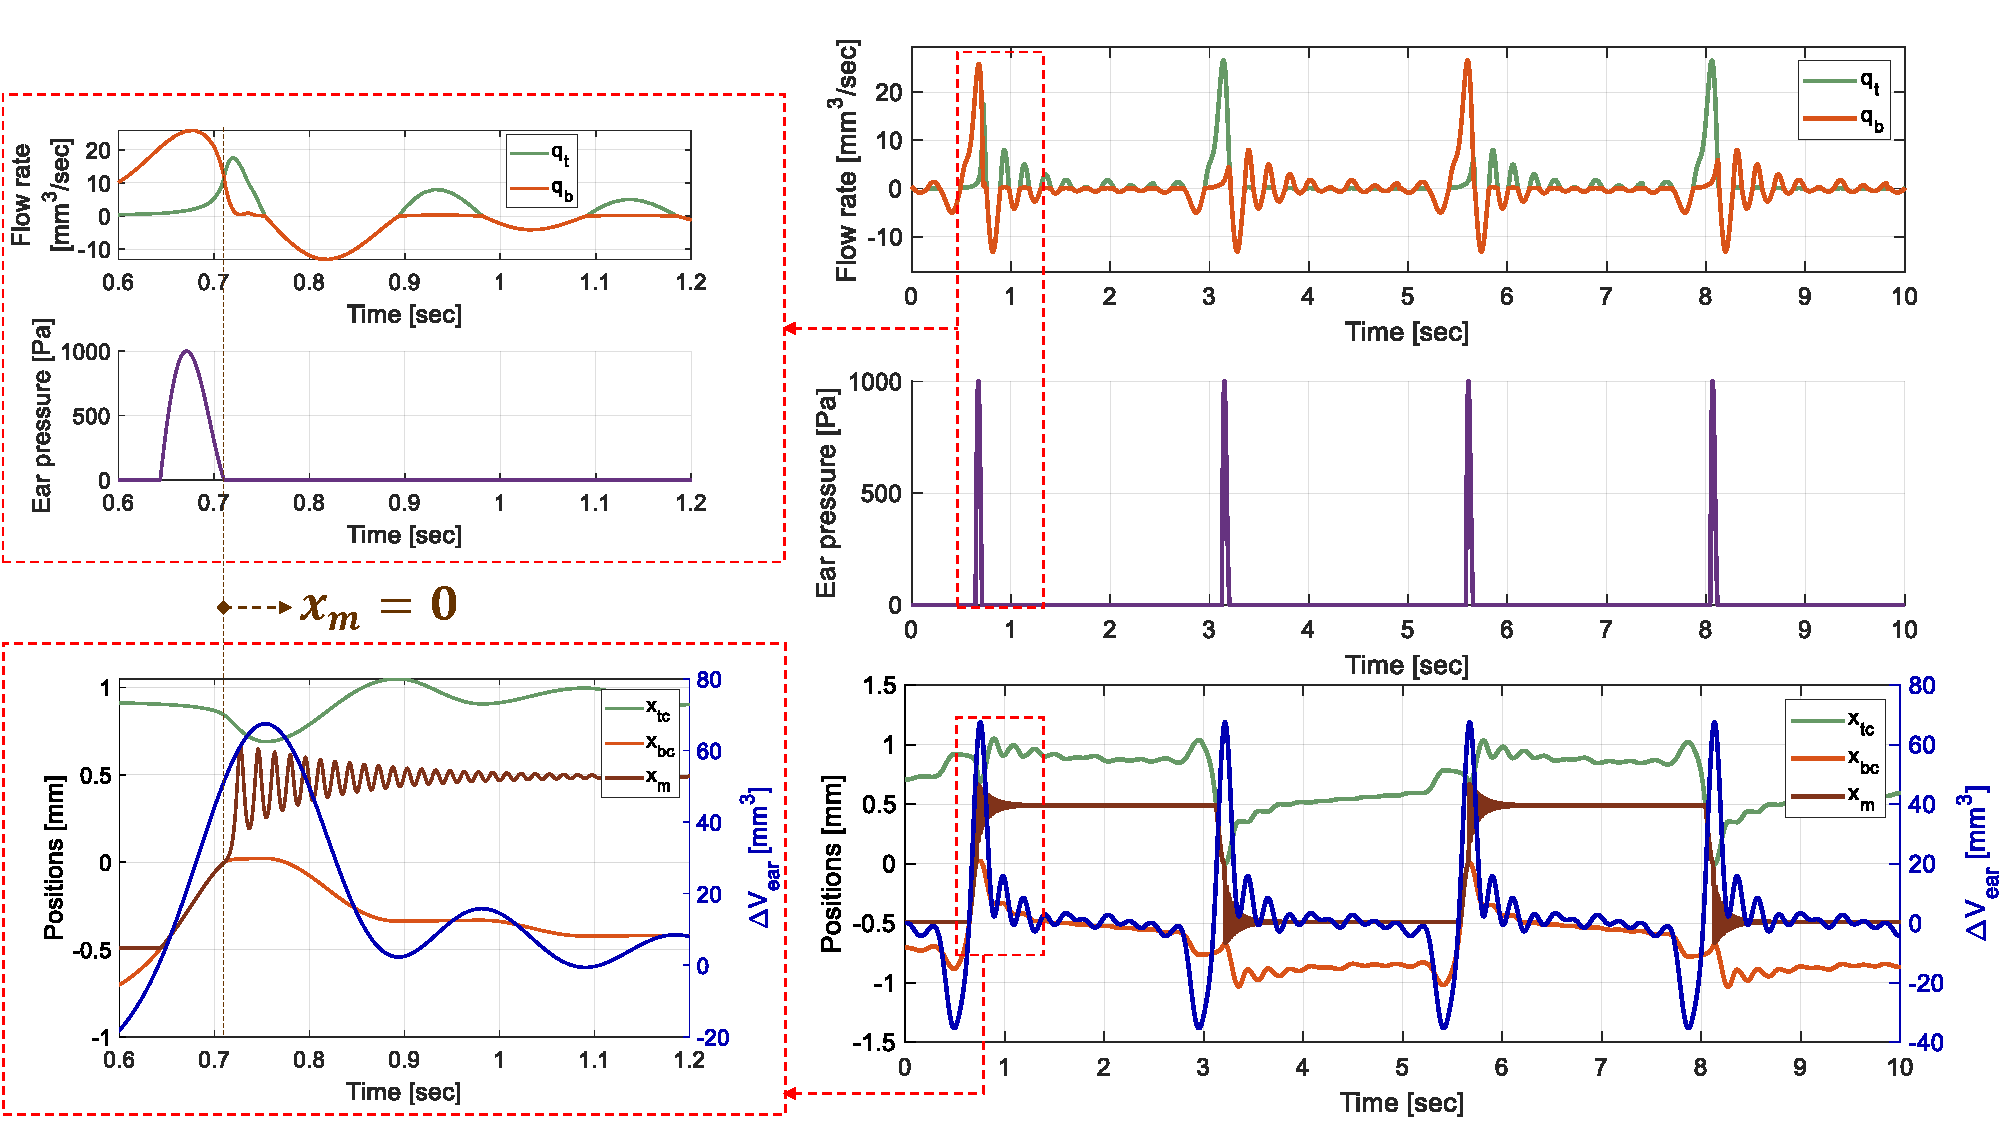
\includegraphics[trim={0cm 0cm 0cm 0.5cm},clip, width=\textwidth]{figures/positions+DeltaV_debits_pear.pdf}
	\caption{}
	\label{fig:positions+DeltaV_debits_pear}
\end{figure*}
%%%%%%%%%%%%%%%%%%%%%%%%%%%%%%%%%%%%%%%
%%%%%%%%%%%%%%%%%%%%%%%%%%%%%%%%%%%%%%
\begin{figure*}[!htbp]
	\centering
	\captionsetup{justification=centering}
	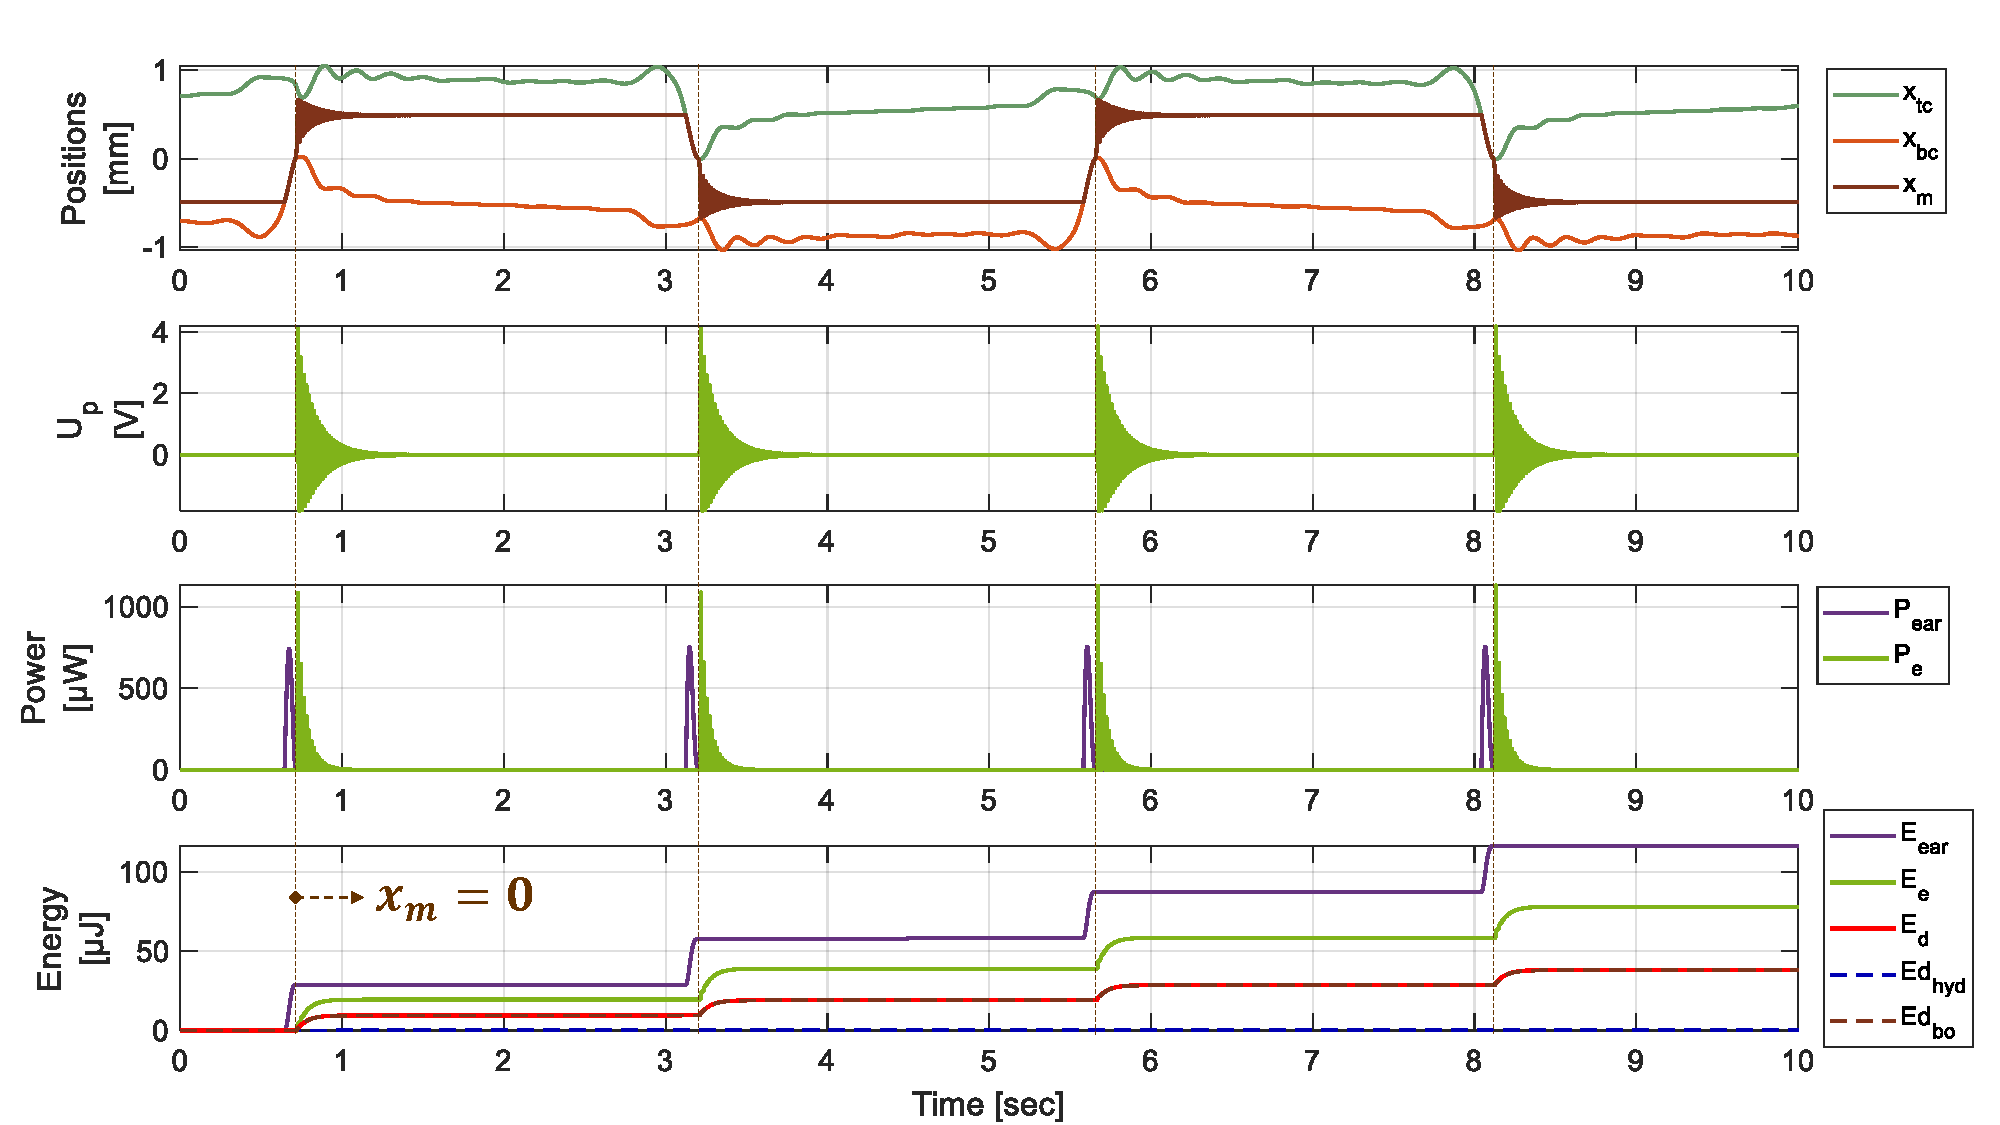
\includegraphics[trim={0cm 0cm 0cm 0cm},clip, width=\textwidth]{figures/positions_Up_puissances_energies.pdf}
	\caption{}
	\label{fig:positions_Up_puissances_energies}
\end{figure*}
%%%%%%%%%%%%%%%%%%%%%%%%%%%%%%%%%%%%%%%
%%%%%%%%%%%%%%%%%%%%%%%%%%%%%%%%%	
\begin{table}
\begin{subtable}[b]{.42\linewidth}
	\centering
	\resizebox{\linewidth}{!}{%
	\begin{tabular}{c|c}
\toprule
\multicolumn{1}{c}{~~\textbf{Parameter}~~}  & \multicolumn{1}{c}{~~\textbf{Value}~~} \\
\midrule
$K_{eq}$	[N/µm]	&	0.256		\\	\hline
$x_0$ [mm]			&	0.49		\\	\hline
$L$	[mm]			&	16.0		\\	\hline
$m$	[g]				&	5.88		\\	\hline
$x_{c0}$ [mm]		&	0.69		\\	\hline
$R_l$ [k$\Omega$] 	&	6.39		\\	\hline
$\alpha$ [N/V]		&   0.105		\\	\hline
$C_p$ [µF]	   		&	0.25		\\	\hline
$Q$ [-]				&	50			\\	\hline
$\eta_g$ [\%]		& 	85			\\
\bottomrule
	\end{tabular}}
	\caption{Electromechanical}
	\label{tab:parametres électromécaniques}			
\end{subtable}
\hfillx
\begin{subtable}[b]{.55\linewidth}
	\centering
	\resizebox{\linewidth}{!}{%
	\begin{tabular}{c|c}
\toprule
\multicolumn{1}{c}{~~\textbf{Parameter}~~}  & \multicolumn{1}{c}{~~\textbf{Value}~~} \\
\midrule
$D_{hc}$ [mm] 	   			&	4						\\ \hline
$a_h$ [-]					&	29			 			\\ \hline
$p_c$ [kPa]					&	1				 		\\ \hline
$(\Delta V{ear})_{max}$ [mm$^3$]	& 60				\\ \hline
$Cf_0$ [Pa.s$^2$/m$^6$]			&	0.21e17			\\ \hline
$r_{Cf}$ [-]						&	26				\\ 
\bottomrule 
	\end{tabular}}
	\caption{Hydraulic}
	\label{tab:parametres_hydrauliques}		
\end{subtable}
\caption{Simulated model theoretical parameters}
\end{table}
%%%%%%%%%%%%%%%%%%%%%%%%%%%%%%%%%

The simulated model shows promising efficiency (tab. \ref{tab:parametres électromécaniques}) and  Next section will present the experimental approach to validate the theoretical behavior of the electromechanical converter.

%/!\/!\/!\/!\/!\/!\/!\/!\/!\/!\/!\/!\/!\/!\/!\/!\/!\/!\/!\/!\/!\/!\/!\/!\%
\section{EXPERIMENTAL CHARACTERIZATION OF THE \mbox{ELECTROMECHANICAL} CONVERTER}
\label{sec:EXPERIMENTAL CHARACTERIZATIONS OF THE ELECTROMECHANICAL CONVERTER}
%/!\/!\/!\/!\/!\/!\/!\/!\/!\/!\/!\/!\/!\/!\/!\/!\/!\/!\/!\/!\/!\/!\/!\/!\%
    %///////////////////////////////////////////// 
	\subsection{Description of the electromechanical converter}	
	\label{Description of the electromechanical converter}
    %/////////////////////////////////////////////
The BR is fabricated by electrical discharge machining (EDM) in a monobloc structure. This method provides better resonator quality factor than when there are assemblies. Figure \ref{fig:BDT_OB+GPA} shows the BR mounted on the experimental test bench. The 8 hinges are ensured using 4 buckled blades (BB) while a vertical guide beam (GB) ensures the APG mounting and prevents any rotations. The local thickenings at the midspan of the blades are intended to facilitate the fabrication. They also maximize the BB compression stiffness that maximizes EH efficiency, as we will explain in the following section. The geometrical and mechanical parameters of the BR are referenced in Table \ref{tab:parametres_lames}. The following sections describe the design method that led to the dimensions of the blades, based on the needs of the application.
%%%%%%%%%%%%%%%%%
\begin{table}[!htbp]
	\centering
    \resizebox{\linewidth}{!}{%
		\begin{tabular}{l|c|c}
			\toprule
\textbf{Parameter definition} & \textbf{Symbol}    & \textbf{Value [Unit]} \\
\midrule
APX4 steel Young's modulus    & $E$                       & 211 [GPa]  \\
APX4 steel elastic resistance & $Re_{APX4}$               & 955[MPa]    \\
Dimensions of a buckled beam  & $L$ x $l$ x $e$           & 16x0.07x1.2 [mm] \\
Dimensions of the guide beam  & $L_{v}$ x $l_{v}$ x $e$   & 17.5x0.07x1.2 [mm] \\
Soft hinge stiffness		  & $K_{\varphi}$             & 0.006 [N.m/rad] \\
Stiffness of the guide beam along $\vec{y}$  & $K_{gb}$   & 190 [N/m] \\
Stiffness of 4 buckled blades along $\vec{z}$ & $K_{bb}$   & 1402 [kN/m] \\  
Stiffness of the APG along $\vec{z}$          & $K$        & 252  [kN/m]\\
			\bottomrule
		\end{tabular}}
	\caption{Definitions and values of the fabricated BR}
	\label{tab:parametres_lames}
\end{table}
%%%%%%%%%%%%%%%%%%%%% 
    %///////////////////////////////////////////// 
	\subsection{Designing the BR beams}	
	\label{subsec:BR beams design}
    %/////////////////////////////////////////////
In the proposed system, energy harvesting occurs at the oscillation phase. The main issue is to maximize the energy conversion efficiency $\eta_{br}$ of this stage. Richards \emph{et al.} demonstrated that for the piezoelectric transduction at the resonance frequency, it can be approximated with Equation \ref{eq:eta_ob} \cite{Richards2004}. This expression is valid for an electric extraction based on the adaptive impedance matching strategy.
\begin{equation}
	\eta_{br} = \dfrac{k^2_{sys}\ Q}{k^2_{sys}\ Q + 2}
	\label{eq:eta_ob}
\end{equation}
where $k^2_{sys}$ is the global electromechanical coupling coefficient of the harvesting system. The latter can be expressed with the electromechanical parameters of the APG and the stiffness of the beams (Table \ref{tab:parametres_lames}) as follows :
\begin{equation}
	k^2_{sys} = \dfrac{\alpha^2_{eq}}{\alpha^2_{eq} + (K+K_{gb})C_p}
	\label{eq:k2_sys}
\end{equation}
where $\alpha_{eq}$ is the equivalent Piezoelectric Force Factor (PFF) given by Equation \ref{eq:alpha_eq}. It depends on the APG PFF and on the ratio between the equivalent stiffness $K_{eq}$ (Eq. \ref{eq:K_eq}) of the structure on the $\vec{z}$ axis and the equivalent stiffness of the APG mounted on the GB.
\begin{equation}
	\alpha_{eq} = \alpha\ \dfrac{K_{eq}}{K + K_{gb}} 
	\label{eq:alpha_eq}
\end{equation}
\begin{equation}
	K_{eq} = \dfrac{K_{bb}(K + K_{gb})}{K_{bb} + K_{gb} + K}
	\label{eq:K_eq}
\end{equation}
Equations \ref{eq:eta_ob} - \ref{eq:K_eq} combined demonstrate that in order to maximize $\eta_{br}$ we must make sure that $K_{bb} \gg K \gg K_{gb}$. If the condition is respected, then $K_{eq}$ can be assimilated to $K$ and $\alpha_{eq} \approx \alpha$.

When the mass crosses the unstable \mbox{$x_m=0$} position, the compression force $F_{z,0}$ induces the maximum stress on the BB. $F_{z,0}$ can be expressed by Equation \ref{eq:Fz0_flambement}. $K_{bb}$ can then be assured if the compression efforts absorbed by the BBs do not induce any secondary buckling mode during the BR operation. 
\begin{equation}
	F_{z,0} = 2K \biggl( \sqrt{x_0^2+L^2}-L \biggr)
	\label{eq:Fz0_flambement}
\end{equation}
The beams design was obtained using a FEM model whose results are summarized in Figure \ref{fig:buckling_limit}. It reveals that the first secondary undesirable buckling mode appears for $F_{z,0}=6.4$\,N. If this happens, the compression force is not transmitted from the mass to the APG, $K_{bb}$ is not assured and $k^2_{sys}$ is diminished (Eq. \ref{eq:k2_sys}). Thus, we establish a buckling height domain (Fig. \ref{fig:buckling_limit}) to avoid the secondary buckling for the fabricated BR. The preliminary simulated case presented in the previous section is in the preferable domain. Moreover, the force absorbed by the APG must be under the maximal limit of $18$\,N above which the device could become damaged.
%%%%%%%%%%%%%%%%%%%%%%%%%%%%%%%%%%%%%%
\begin{figure}[!htbp]
	\centering
	\captionsetup{justification=centering}
	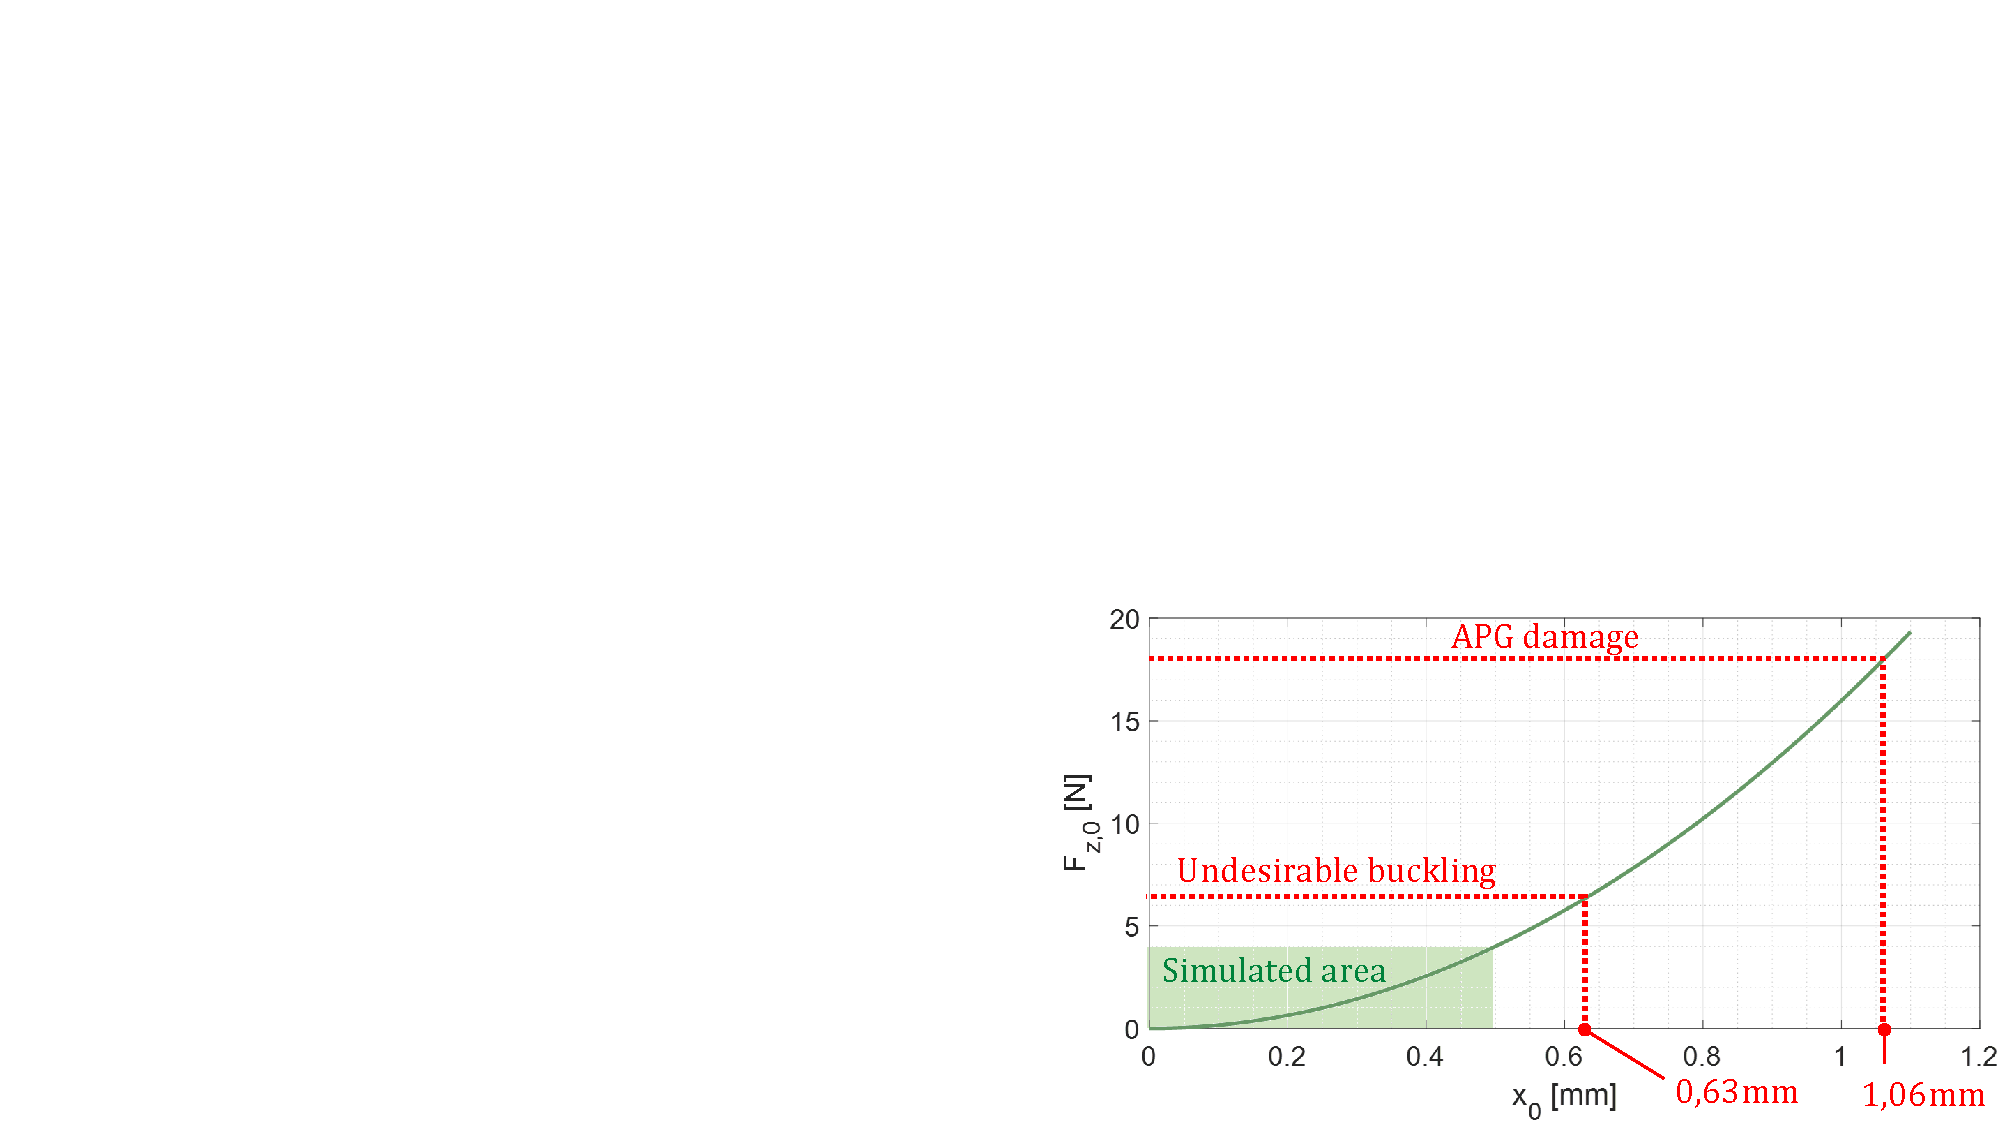
\includegraphics[trim={17.9cm 0cm 0cm 10cm},clip,width=0.9\linewidth]{figures/buckling_limit.pdf}
	\caption{APG elastic counter reaction on $\vec{z}$ axis at $x_m=0$, depending on the initial structural buckling height $x_0$}
	\label{fig:buckling_limit}
\end{figure}
%%%%%%%%%%%%%%%%%%%%%%%%%%%%%%%%%%%%%%
% Ltex language=en

    %///////////////////////////////////////////// 
	\subsection{Experimental characterizations}	
	\label{subsec:Experimental characterizations}
    %/////////////////////////////////////////////
The experimental test bench for the characterizations of the electromechanical converter is presented in Figure \ref{fig:BDT_OB+GPA}. An additional beam is mounted with the APG to prevent any rotation whatsoever. A micrometric screw sets the initial buckling level to $x_0$ ($\pm 10$\,µm). The bearing decouples the rotation of the screw with the beam structure to prevent unwanted torsional stress. The central mass at $\degree{45}$ receives and reflects the displacement sensor emitted laser along the $\vec{z}$ axis and captures the $x_m$ position. The APG power is dissipated in the $R_l$ resistor and the $U_p$ voltage ($\pm 1$\,mV), along with $x_m$, are monitored through a data acquisition card NI-USB 6212 and a LabVIEW interface. Finally, the two HC plungers actuate the mass from one stable equilibrium position to the other. The HV mechanical influence is not considered here in order to focus on the electromechanical converter dynamic behavior. 
%%%%%%%%%%%%%%%%%%%%%%%%%%%%%%%%%%%%%%
\begin{figure}[!htbp]
	\centering
	\captionsetup{justification=centering}
	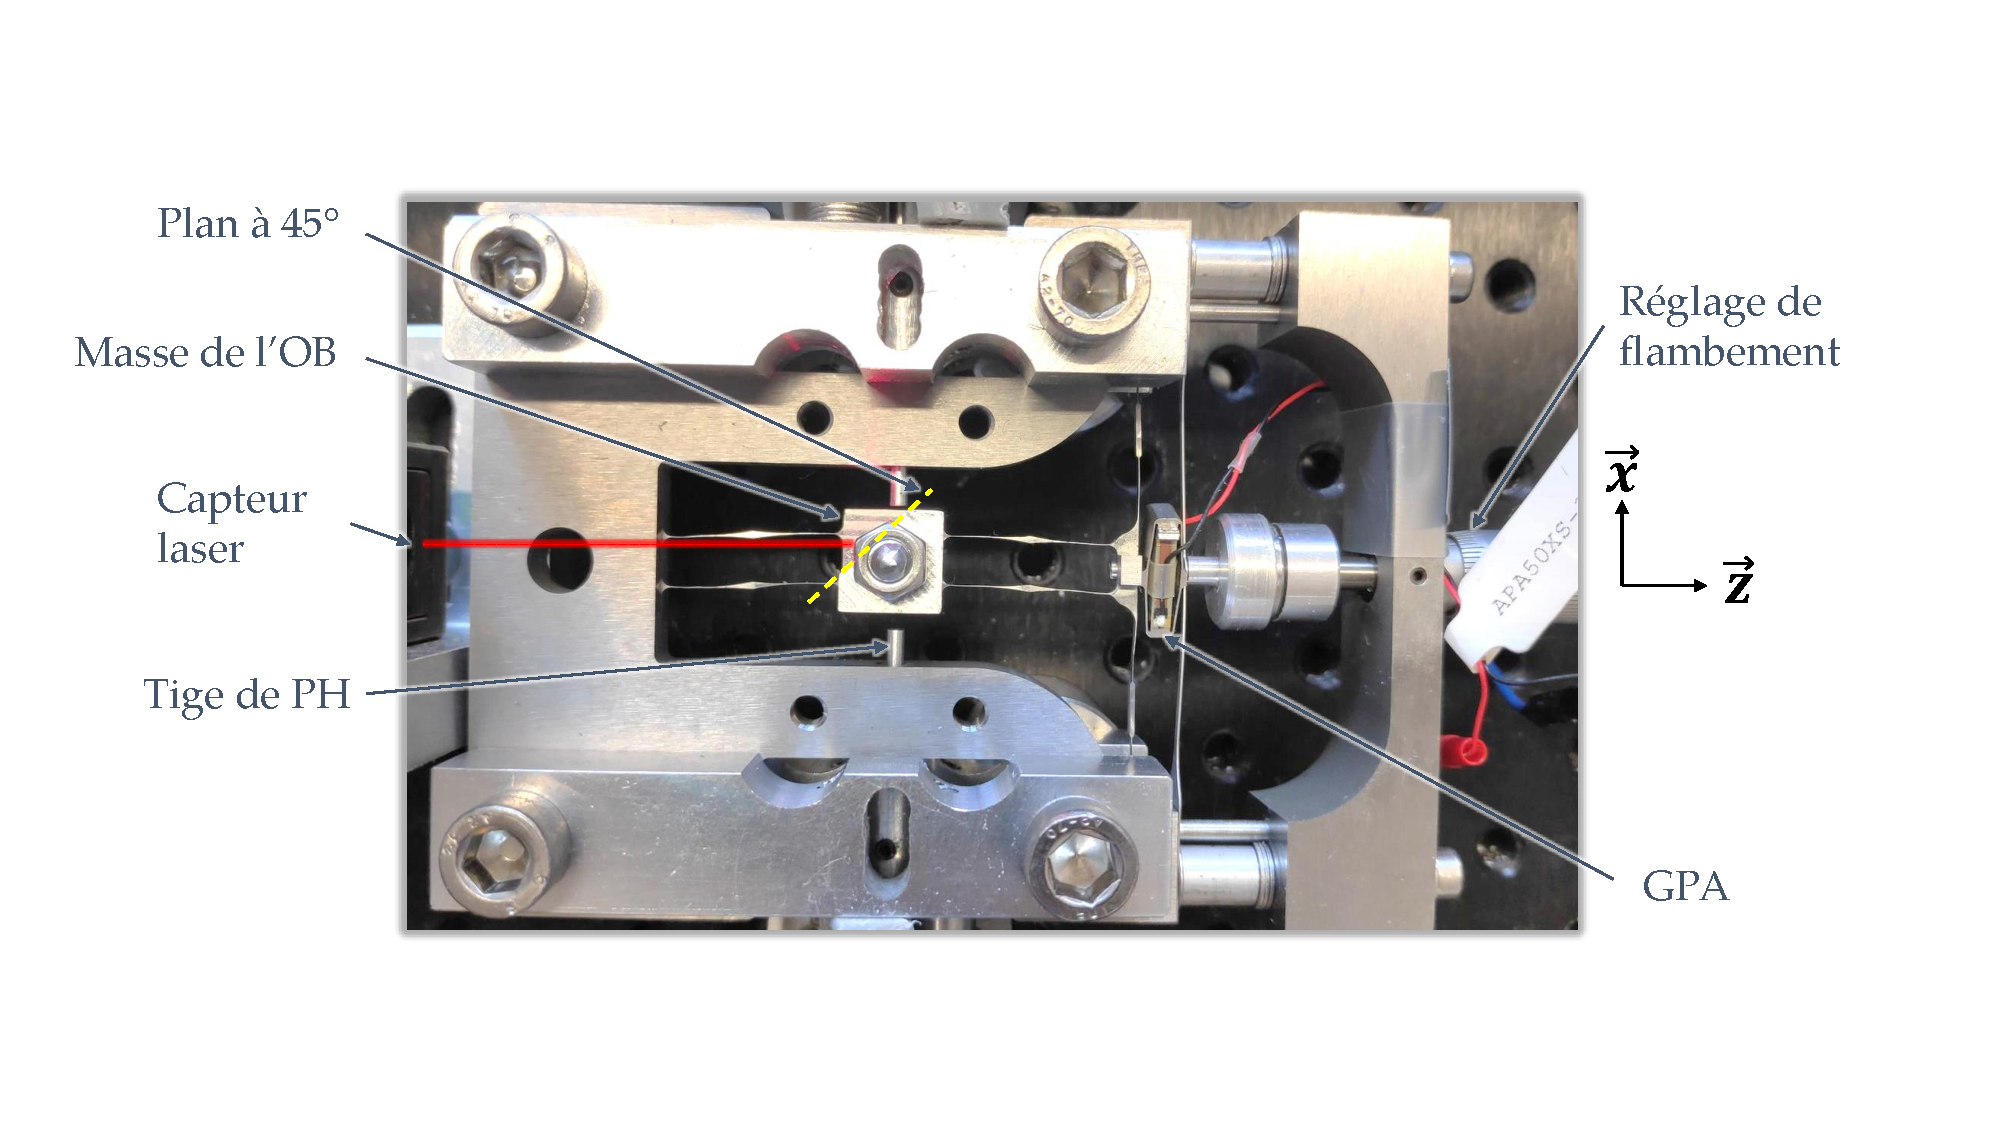
\includegraphics[trim={2cm 0cm 0cm 5.5cm},clip,width=\linewidth]{figures/BDT_OB+GPA.pdf}
	\caption{Test bench of the electromechanical converter}
	\label{fig:BDT_OB+GPA}
\end{figure}
%%%%%%%%%%%%%%%%%%%%%%%%%%%%%%%%%%%%%%%

The mass is pushed by a HC from a stable equilibrium position until it reaches \mbox{$x_m=0$}, and then oscillates around the opposite stable equilibrium position. The experimental data have been fitted on the oscillation phase of the simulated global model as the test bench does not reproduce the hydraulic circuit behavior yet. This data was used to identify and recalibrate the following electromechanical parameters of the EH, through iterative simulations of the global \mbox{model :} $Q$, $f_0$, $K$ and $k_{sys}^2$ (Table \ref{tab:parametres_lacher_free}).  The experimental oscillation frequency $f_0$ and energy conversion efficiency $\eta_{br}$ were also calculated.
%%%%%%%%%%%%%%%%%
\begin{table}[!htbp]
\centering
\captionsetup{justification=centering}
\resizebox{.8\linewidth}{!}{%
	\begin{tabular}{ c | c | c }
	\toprule
	& \textbf{Simulation with}  	   & \textbf{Simulation with}       \\
	& \textbf{theoretical}  		   & \textbf{recalibrated }		 	\\
	\multirow{-3}{*}{\textbf{Symbol}}
	& \textbf{parameters}			   & \textbf{parameters} 			\\
	\midrule
	$Q$                       & 50.0                  & 30.0 		  	\\  
	$f_0$                     & 47.0 Hz               & 27.9 Hz  		\\
	$x_0$                     & 0.49 mm               & 0.50 mm    		\\
	$K_{eq}$                  & 2.56e5 N/m            & 0.85e5 N/m 		\\
	$K_{bb}$                  & 14.2e5 N/m            & 1.27e5 N/m 		\\
	${k^2_{sys}}$             & 16 \%                 & 1.25 \% 		\\
	$\eta_{br}$               & 85 \%                 & 12.9 \%   		\\
	\bottomrule
	\end{tabular}}
	\caption{Theoretical and experimentally recalibrated values of the electromechanical converter's parameters.}
	\label{tab:parametres_lacher_free}
\end{table}  
%%%%%%%%%%%%%%%%%%%%%  

Experimental $K_{bb}\approx K/2$ can be calculated from the identified $K_{eq}$ with Equation \ref{eq:K_eq}, supposing $K_{gb}$ is negligible (Table \ref{tab:parametres_lames}).
    %///////////////////////////////////////////// 
	\subsection{Analysis and summary}	
	\label{subsec:Analyze and summary}
    %/////////////////////////////////////////////
The experimental dynamic behavior of the converter is predictable using the equations established once the system parameters, listed in Table \ref{tab:parametres_lacher_free} had been identified. However, the performances of the experimental prototype are below the theoretical expectations (Table \ref{tab:parametres électromécaniques}). This efficiency discrepancy is mainly associated with the quality factor and the electromechanical coupling coefficient drop (Eq. \ref{eq:eta_ob}). 

The decrease in quality could be related to the general non-permanent assembly that uses non-perfect embeddings with fixation screws and a mobile micrometric screw. Small undulations were observed on the BBs after fabrication and may also have gotten worse during the manipulation. These undulations increase the probability of secondary buckling which contribute to reducing $K_{bb}$ and diminishing $k^2_{sys}$, according to Equations \ref{eq:k2_sys}-\ref{eq:K_eq}. Improvements are proposed further on to resolve this issue and reduce the energy losses during this stage.

%/!\/!\/!\/!\/!\/!\/!\/!\/!\/!\/!\/!\/!\/!\/!\/!\/!\/!\/!\/!\/!\/!\/!\/!\%
\section{EXPERIMENTAL APPROACH FOR THE HV \mbox{DESIGN}}
\label{sec:EXPERIMENTAL APPROACH FOR THE HV DESIGN}
%/!\/!\/!\/!\/!\/!\/!\/!\/!\/!\/!\/!\/!\/!\/!\/!\/!\/!\/!\/!\/!\/!\/!\/!\%
To validate the feasibility of the HVs, we adopted an experimental approach to find the material and geometrical parameters of the tube to achieve $(r_{Cf})_{min}=26$ (Tab. \ref{tab:parametres_hydrauliques}). A buckled kapton tube \cite{Dupont2012} of internal diameter $D_t=1.05$\,mm and thickness $th_t=25$\,µm was found to meet this hydraulic criteria. It will be referred to as HV$_{T1}$. 
    %///////////////////////////////////////////// 
	\subsection{HV hydraulic experimental characterization}	
	\label{subsec:HV hydraulic test bench presentation}
    %/////////////////////////////////////////////
Figure \ref{fig:essais_hydraulique_VH} shows the HV$_{T1}$ during the experimental characterizations on the hydraulic test bench. An electromechanical rotary plate is monitored on the LabVIEW interface and imposes a bending angle $\theta$. A liquid-filled syringe sets the fluid flow through the HV$_{T1}$ and $q_{syr}$ is evaluated by tracking the syringe piston displacement. The pressure loss coefficient $Cf_{T1}$ is calculated as \mbox{follows:}
\begin{equation}
	Cf_{T1} = \dfrac{p_1-p_2}{q_{syr}^2}
\end{equation}
where $p_1$ and $p_2$ are the fluid pressures monitored before entering and after exiting the HV$_{T1}$ respectively.
%%%%%%%%%%%%%%%%%%%%%%%%%%%%%%%%%%%%	
\begin{figure*}[!htb]
\begin{center}
	\captionsetup{justification=centering} 
	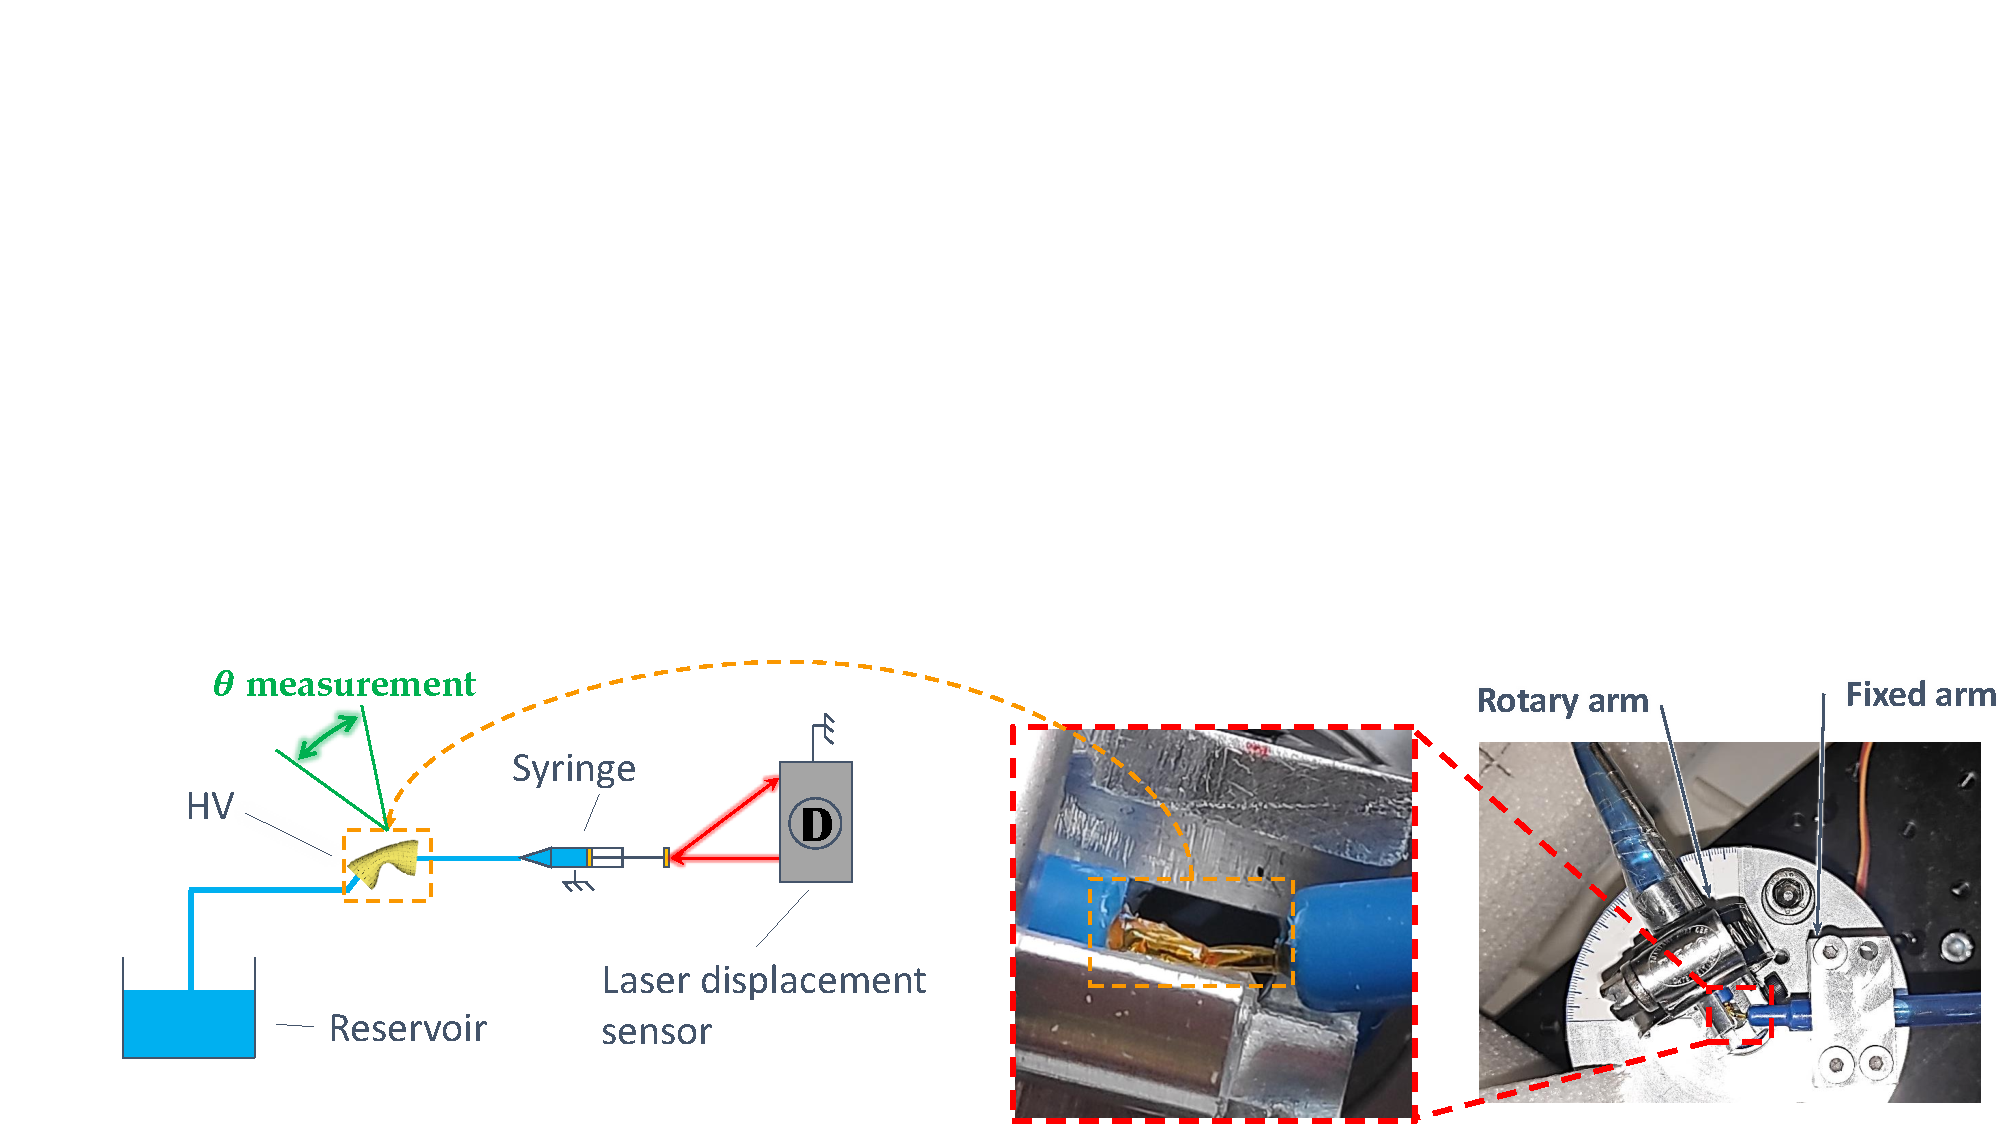
\includegraphics[trim={2cm 0cm 0cm 11cm},clip,width=.8\textwidth]{figures/essais_hydraulique_VH.pdf}
	\caption{Hydraulic characterization test bench for HVs}
	\label{fig:essais_hydraulique_VH}
\end{center}	
\end{figure*}    
%%%%%%%%%%%%%%%%%%%%%%%%%%%%%%%%%%%% 
The tests were repeated 7 times for $\theta$ varying from $0^{\circ}$ to $60^{\circ}$ with $10^{\circ}$ increments. The experimental results are plotted on Figure \ref{fig:resultats_essais_hydraulique_VH_D1mm}.
%%%%%%%%%%%%%%%%%%%%%%%%%
\begin{figure}[!htbp]
\centering
	\captionsetup{justification=centering}
	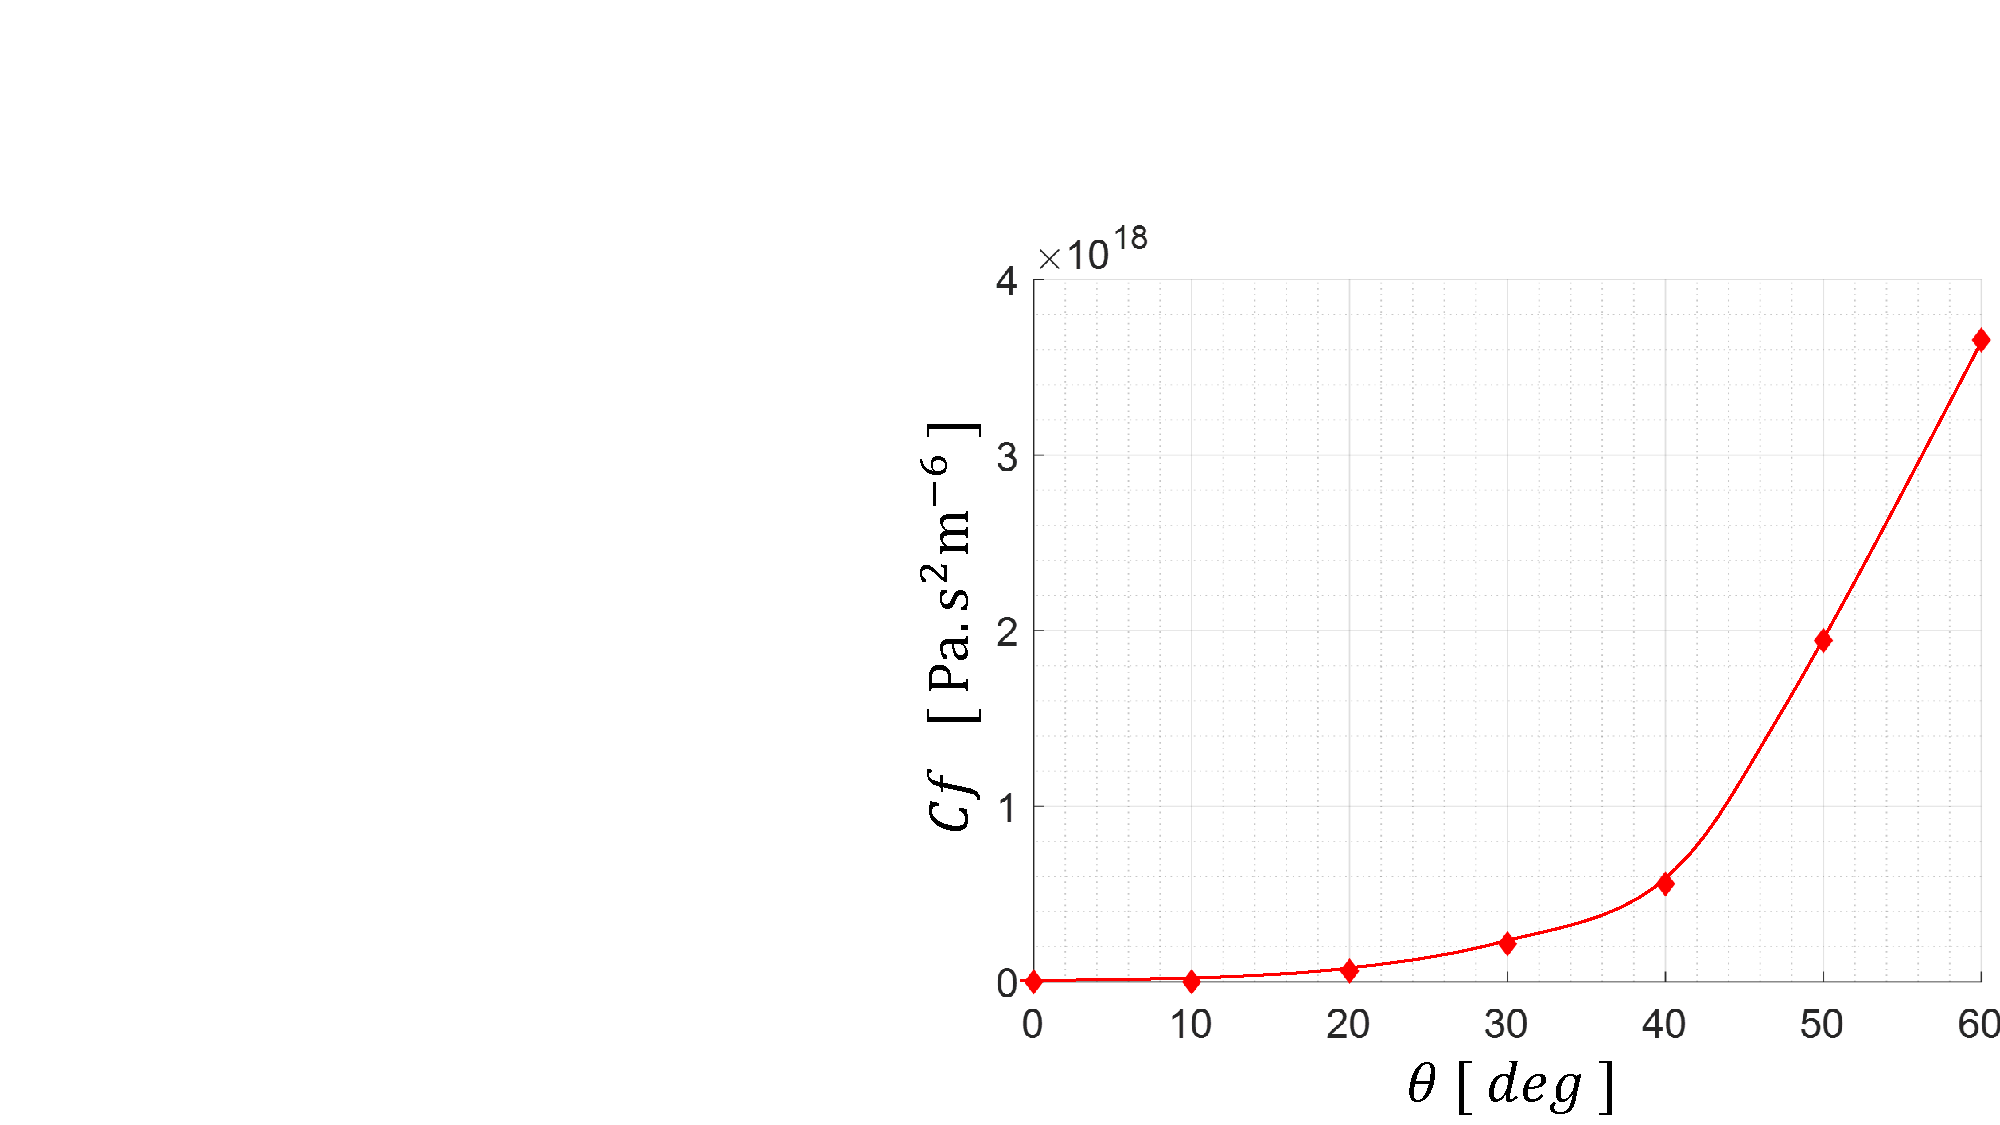
\includegraphics[trim={15.5cm 0cm 0cm 3.6cm},clip,width=0.6\linewidth]{figures/resultats_essais_hydraulique_VH_D1mm.pdf}
	\caption{Hydraulic characterization of the HV$_{T1}$.}
	\label{fig:resultats_essais_hydraulique_VH_D1mm}
\end{figure}
%%%%%%%%%%%%%%%%
The hydraulic restriction coefficient of the HV$_{T1}$ has been evaluated to $r_{Cf}60$ if we consider the opened angle $\theta_0=20^{\circ}$ and the closed angle $\theta_c = 60^{\circ}$. Its hydraulic behavior respects the minimum criteria of \mbox{$(r_{Cf})_{min}=26$} and therefore can ensure the adequate hydraulic commutation to cycle the BR mass motion. In order to set an optimal angle operation range $\Delta\theta$, we must investigate the evolution $K_{HV}(\theta)$. This will not be discussed in this paper. However, $\Delta\theta$ must be minimized in order to limit the energy needed for the HV's operation and also, $\theta_0$ must be minimized to reduce the hydraulic energy losses in the active branch.

The following section presents the EH model using the hydraulic characterization data of the HV$_{T1}$ and the electromechanical experimental data of the BR with the APG.

%/!\/!\/!\/!\/!\/!\/!\/!\/!\/!\/!\/!\/!\/!\/!\/!\/!\/!\/!\/!\/!\/!\/!\/!\%
\section{GLOBAL MODEL RECALIBRATION WITH \mbox{EXPERIMENTAL} DATA}
\label{sec:MODEL RECALIBRATION WITH EXPERIMENTAL DATA}
%/!\/!\/!\/!\/!\/!\/!\/!\/!\/!\/!\/!\/!\/!\/!\/!\/!\/!\/!\/!\/!\/!\/!\/!\%
The experimentally identified parameters have been implemented in the global multiphysics coupled model to enhance its predictability and to evaluate the EH performances. The mechanical influence of the HV$_{T1}$ is identified with an experimental approach, characterizing the energy losses at the HV-mass contact point (T on Figure \ref{fig:HV_actuation_detail}). 
	%/////////////////////////////////////////////
	\subsection{Recalibration with release trials}
	%/////////////////////////////////////////////
The HV$_{T1}$ was mounted onto the experimental test bench presented in Figure \ref{fig:BDT_OB+GPA} and two experimental trials were performed to identify the HV mechanical influence: free oscillations and oscillations with the presence of the HV$_{T1}$, during a harvesting phase. Thus, the difference in the dynamics between the two tests focuses on the HV$_{T1}$'s mechanical influence. 

The mass is initially set to $x_m=x_0$ and then pushed toward $x_0$. The HV$_{T1}$'s internal pressure is adjusted to $30$\,kPa with an oil column, in order to be consistent with the simulated case (Tab. \ref{tab:parametres_hydrauliques}). The oscillation phase begins when the mass crosses the $x_m=0$ position. In order to set $\theta_0$, we added two angle stoppers, illustrated in Figure \ref{fig:contact_M_VH_lachers}. $\theta_c$ is then reached when the oscillations stop at $x_m=x_0$. The mass position and the APG tension were monitored during the tests.
%%%%%%%%%%%%%%%%%%%%%%%%%%%%%%%%%%%%	
\begin{figure}[!htbp]
	\begin{center}
		\captionsetup{justification=centering}
		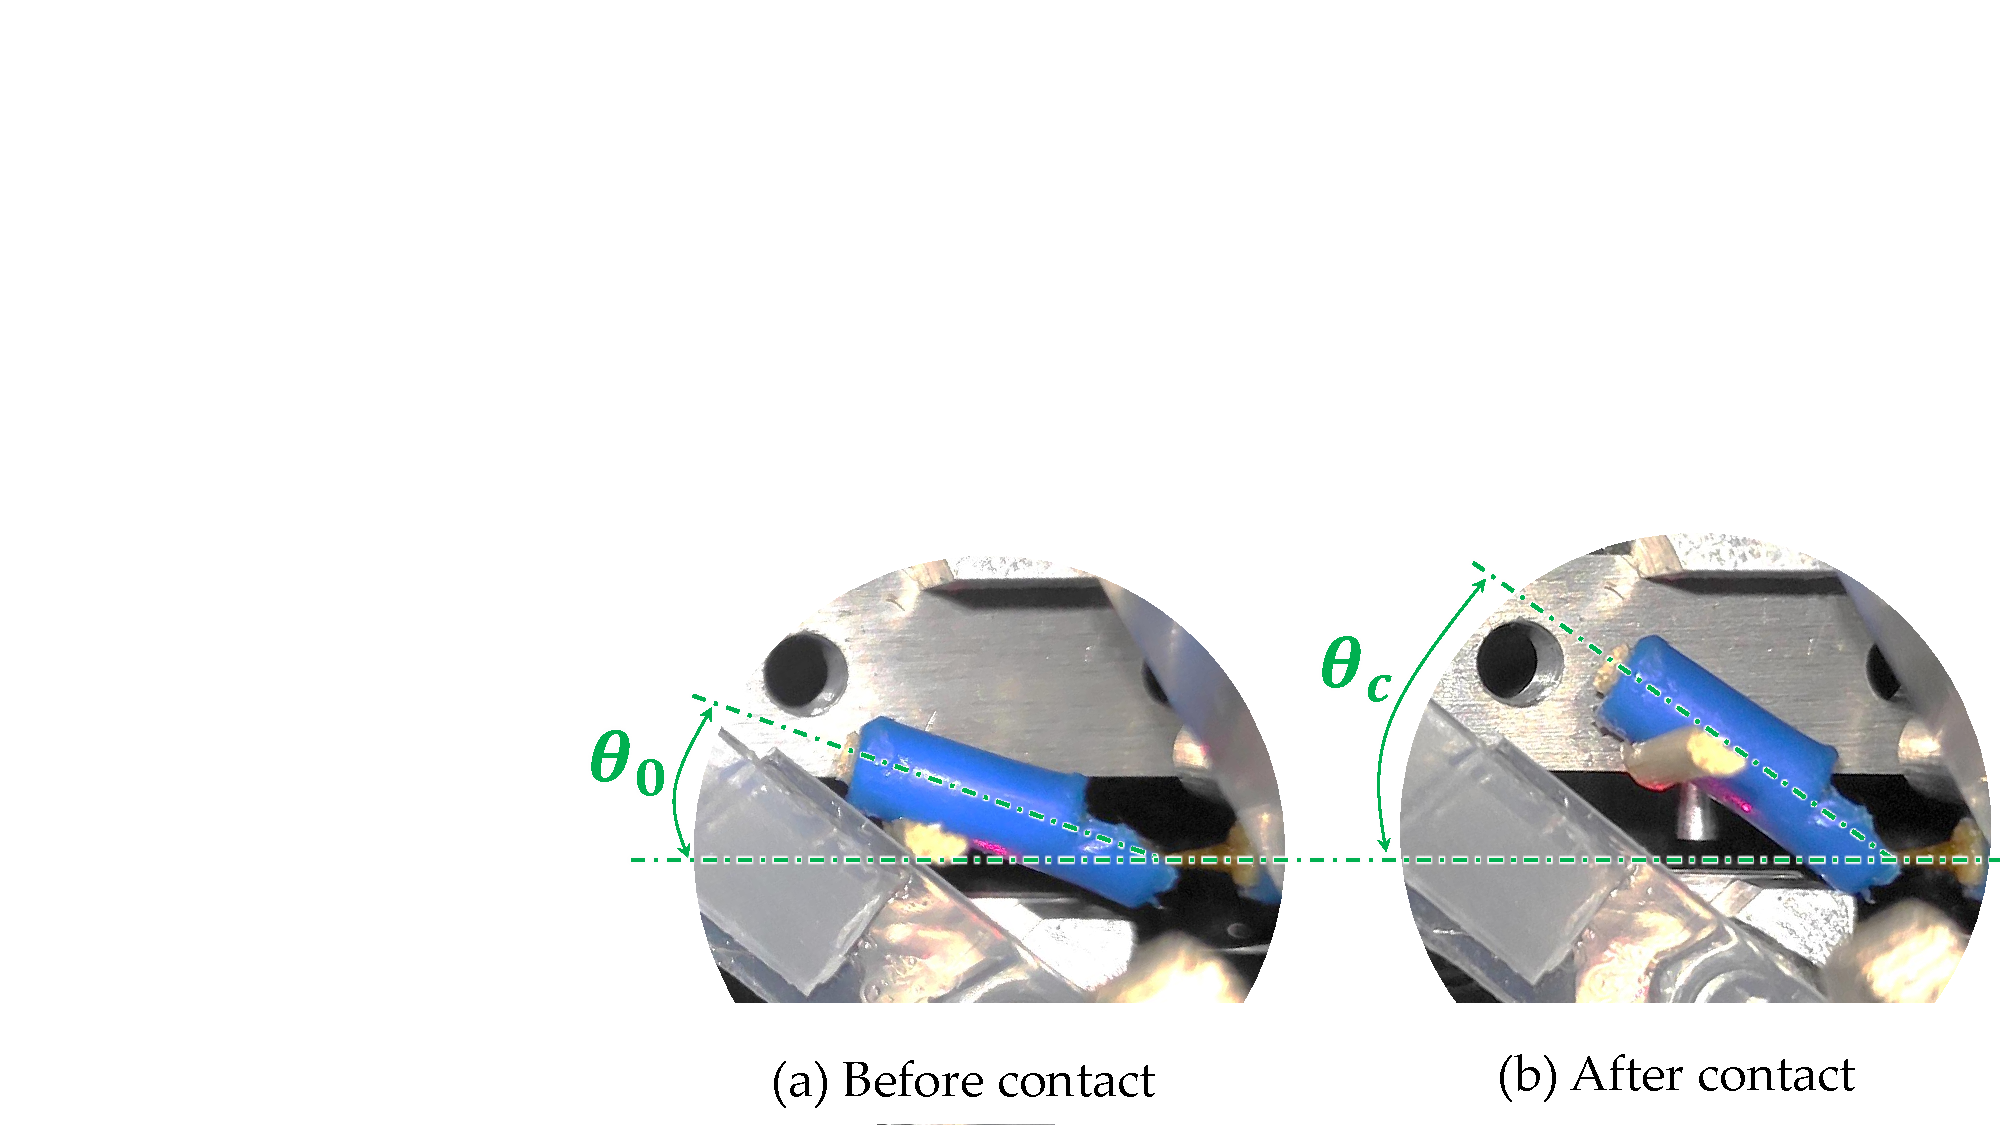
\includegraphics[trim={6.9cm 0cm 0cm 9cm},clip,width=0.9\linewidth]{figures/contact_M_VH_lachers.pdf}
		\caption{HV$_{T1}$ picture for (a).$\theta_0(x_m=-x_{0})$ and for (b).$\theta_f(x_m=x_0$).}
		\label{fig:contact_M_VH_lachers}
	\end{center}
\end{figure}
%%%%%%%%%%%%%%%%%%%%%%%%%%%%%%%%%%%%

The global model parameters listed in Table \ref{tab:parametres lacher tube} are recalibrated for both test configurations by iterative simulations. The simulations with the recalibrated parameters and the experimental data are superimposed on Figure \ref{fig:recalage_global} concerning the harvesting phase of both configurations. 

After recalibration, the good match between the simulated and the experimental data verify that the electromechanical dynamic behavior of the EH is theoretically predictable by the established model. The HV$_{T1}$ stiffness shifts $x_0$ toward $0$ and its value at $\theta_c$ is evaluated with the shift gap and Equation \ref{eq:OB-GPA}. The HV$_{T1}$ adds a supplementary dynamic mass in the BR and changes the oscillation frequency. The electromechanical coupling coefficient is not influenced by the presence of the HV. The quality factor decreases and the dry friction coefficient is calculated from the drop. Moreover, $a$ and $\Delta\theta$ are graphically evaluated.
%%%%%%%%%%%%%%%%%%%%%%%%%%%%%%%%%%%%%%
\begin{figure}[!htbp]	
\captionsetup{justification=centering}
	\begin{subfigure}{.49\linewidth}
		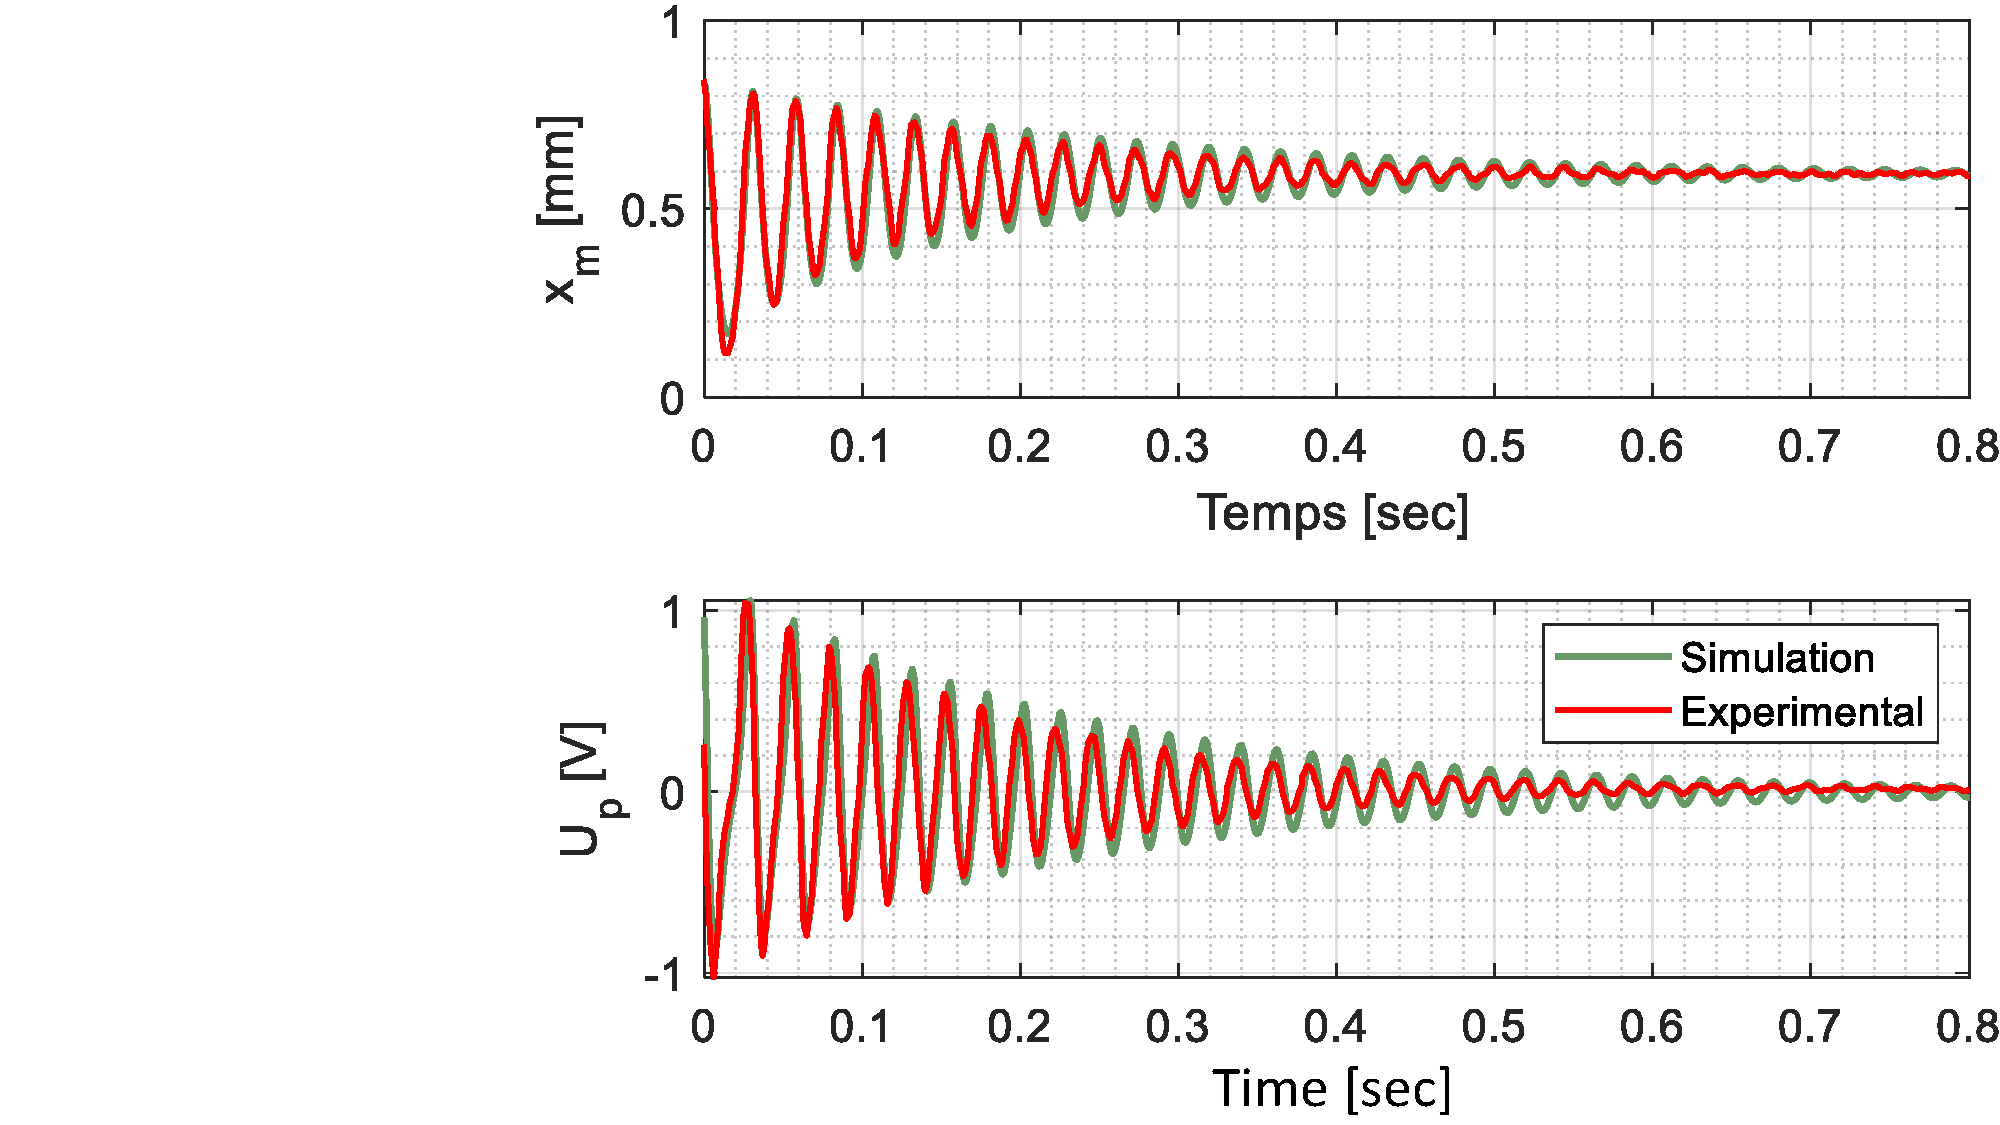
\includegraphics[trim={9cm 0cm 0cm 0cm},clip,width=\linewidth]{figures/recalage_free.pdf}
		\caption{Free oscillations}
		\label{fig:recalage_free}
	\end{subfigure}
	\begin{subfigure}{.49\linewidth}
		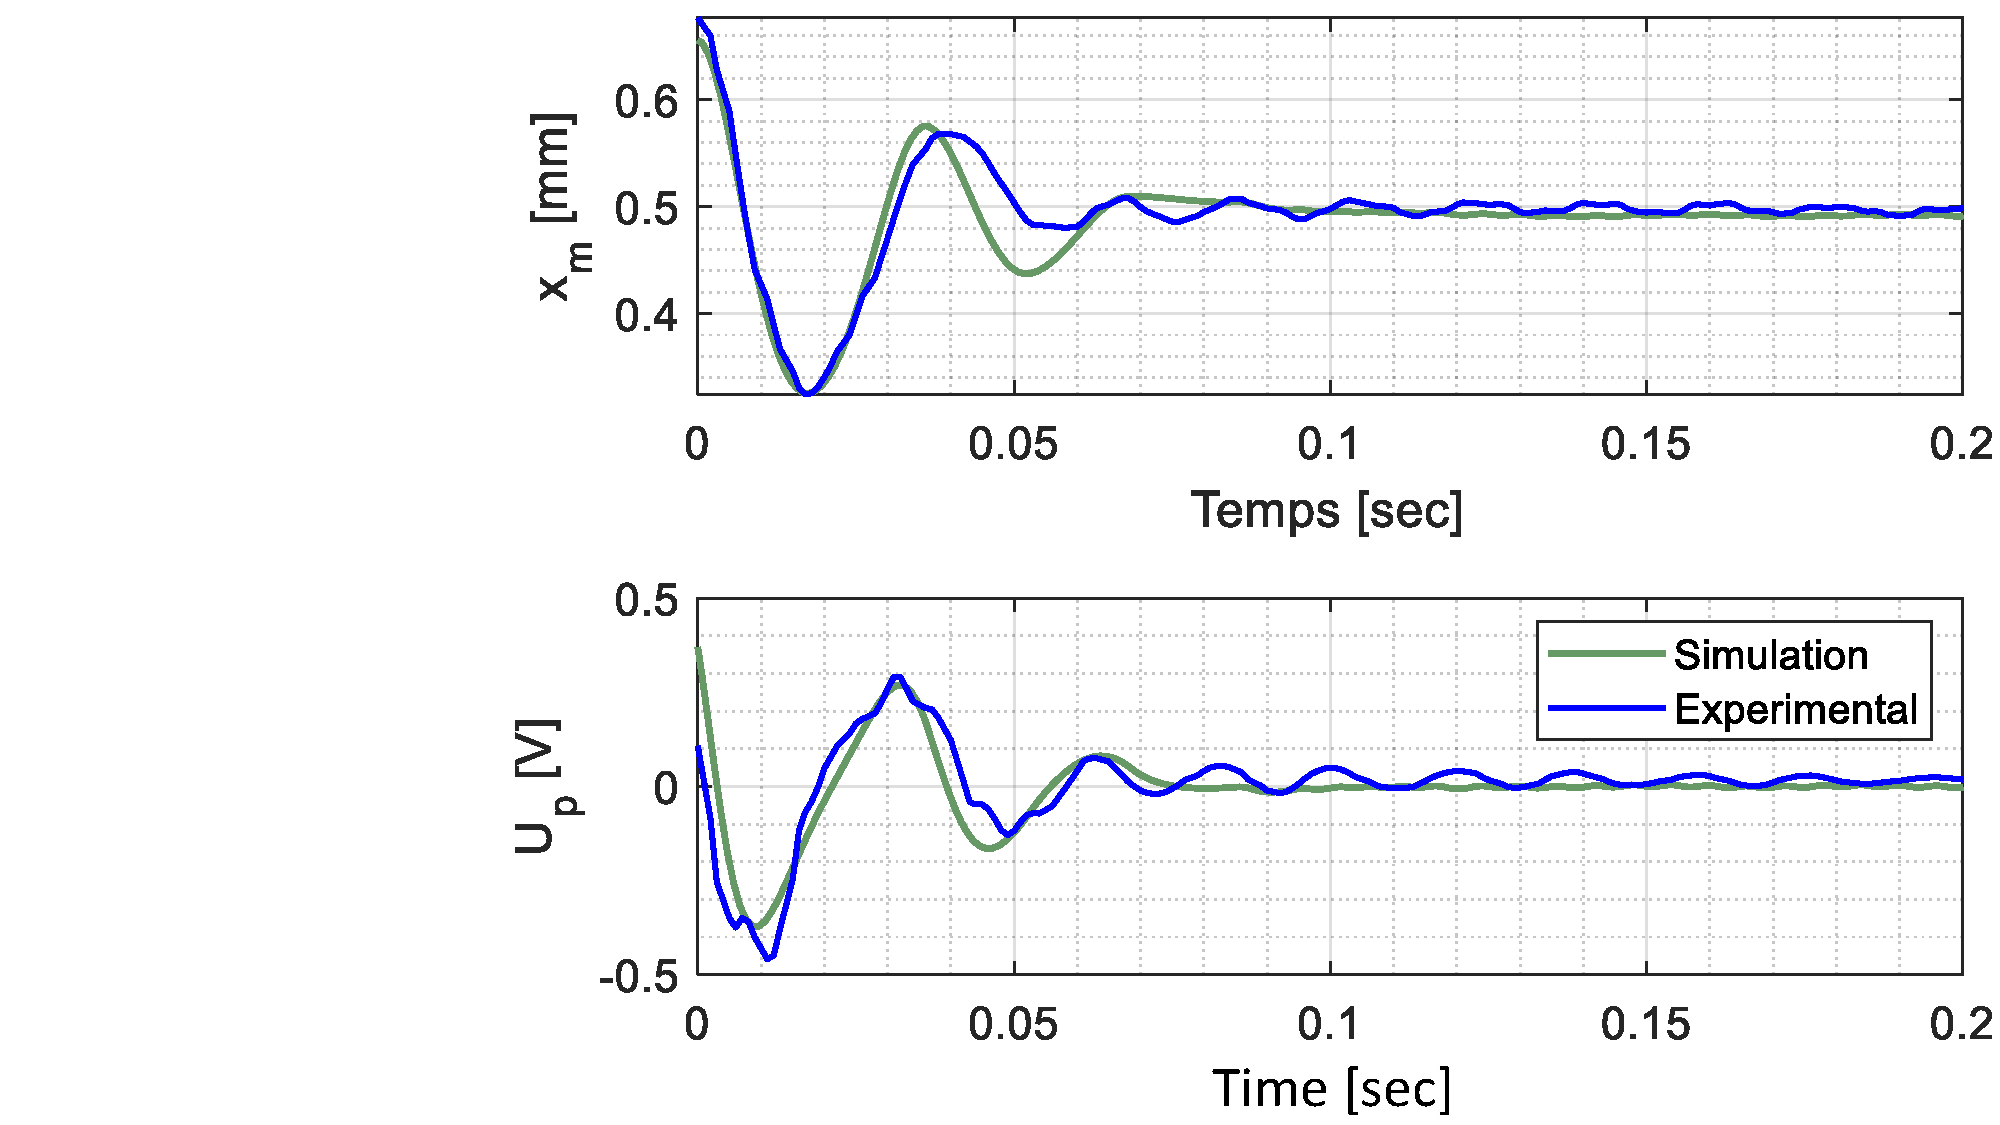
\includegraphics[trim={8.6cm 0cm 0cm 0cm},clip,width=\linewidth]{figures/recalage_tube.pdf}
		\caption{Oscillations with HV$_{T1}$ presence}
		\label{fig:recalage_tube}
	\end{subfigure}
	\caption{Experimental measurements and global system simulation with the identified parameters of Table \ref{tab:parametres lacher tube}.}
	\label{fig:recalage_global}
\end{figure}
%%%%%%%%%%%%%%%%%%%%%%%%%%%%%%%%%%%%%%%
%%%%%%%%%%%%%%%%%%%%%%%%%%%%%%%%%%%
\begin{table}[!htbp]
	\centering
	% \resizebox{\textwidth}{!}{%
		\begin{tabular}[t]{c|c|c}
\toprule
\multicolumn{1}{c}{\textbf{Parameter}}	&
\multicolumn{1}{c}{\textbf{BR}} 	& 
\multicolumn{1}{c}{\textbf{BR+HV$_{T1}$}}  \\
\midrule
$D_r$ [mm] 						& \cellcolor{ashgrey} 		& {4} 		\\ \hline
$\Delta\theta$ [deg] 			& \cellcolor{ashgrey} 		& {{[$\approx$ 19 ; $\approx$ 36]}} \\ \hline
$K_{T1}(\theta_c)$ [Nmm/rad]	& \cellcolor{ashgrey}  		&  0.27 		\\ \hline
$a$ [mm]         			    & \cellcolor{ashgrey}  		&  2.24		\\ \hline
$f_d$ [-] 						& \cellcolor{ashgrey}  		&  0.42  		\\ \hline
$K$ [N/m] 						&	84480			  	 	&  84480  			\\ \hline
$x_0$ [mm] 						& {0.59}					& {0.50}  	\\ \hline
$Q$	[-] 						& 		24.0		 		& 5.0     					\\ \hline
$k^2_{sys}$ [\%] 				& 		1.25		 		& {1.25}   	\\ \hline
$\eta_{br}$ [\%] 				& 		12.9		 		& 2.6   \\ \hline	
$R_l$ [k$\text{\ohm}$] 			&	{15.5}					& {15.5}   	\\ \hline		
$m$	[g]						    &	{5.88}					& 9.00   		\\ \hline	
$f_0$ [Hz]						&		32.9				& 27.9   					\\
\bottomrule	
	\end{tabular}
        \caption{Experimentally recalibrated values of the EH parameters with and without the presence of the HV$_{T1}$.}
        \label{tab:parametres lacher tube}
\end{table}        
	%/////////////////////////////////////////////
	\subsection{Analysis and discussion}
	%/////////////////////////////////////////////
The experimental hydraulic behavior of the HV$_{T1}$ is theoretically capable of providing \mbox{$r_{Cf}>26$} and ensuring an adequate hydraulic commutation cycling for the BR mass's motion.

The quality factor decrease is due to the rubbing between the mass and the HV and diminishes the BR energy conversion efficiency. The friction losses can be minimized by an order of magnitude by using materials with low friction coefficient, like teflon \cite{Nosonovsky2013}. The HV-mass contact can also profit from magnetic interactions instead of direct rubbing.

The global electromechanical coupling is not influenced by the presence of the HV, which is consistent with Equation \ref{eq:k2_sys}. Most of the energy loss is due to the $k^2_{sys}$ drop as a result of the softening of the BBs from the prototype fabrication and manipulation. It can be minimized by using thicker BBs while taking care that the buckling domain does not reach the critical point where the APG could be damaged (Fig. \ref{fig:buckling_limit}). With BBs having a thickness of $200$\,µm instead of $75$\,µm, we can expect 26\,\% improvement on $\eta_{br}$ (Eqs. \ref{eq:eta_ob}-\ref{eq:K_eq}).
%%%%%%%%%%%%%%%%%%%%%%%%%%%%%%%%%%%%	
%/!\/!\/!\/!\/!\/!\/!\/!\/!\/!\/!\/!\/!\/!\/!\/!\/!\/!\/!\/!\/!\/!\/!\/!\%
\section{CONCLUSION}
\label{sec:CONCLUSION}
%/!\/!\/!\/!\/!\/!\/!\/!\/!\/!\/!\/!\/!\/!\/!\/!\/!\/!\/!\/!\/!\/!\/!\/!\%
This work emphasizes the need to enhance the autonomy of the batteries of devices such as hearing aids and the exploitation of the mechanical deformation of the earcanal as a solution.

A new EH architecture maximizing the energy conversion efficiency is proposed. A hydraulic, mechanical and electrical coupled model is established. Its numerical evaluation predicts that the system can theoretically harvest 85\% of the available energy with a hydraulic extraction method. The dynamic behavior and the performances of the fabricated electromechanical converter composed of a BR and APG are evaluated. A new concept of HVs is proposed, based on the buckling of flexible tubes. The proposed HV design is further investigated experimentally to verify if the required theoretical behavior extracted from the numerical simulations is achieved.

The experimental data was used to recalibrate the EH multiphysics model and to evaluate its performances. The global predicted efficiency is $\eta_g=2.6\,\%$. The energy losses factors are identified and solutions are proposed to increase the efficiency to 26\%.

\section{Acknowledgments}
The authors would like to thank Jacob Bouchard-Roy for the data on jaw-joint hydraulic source as well as Michel Demuynck for the constructive exchanges on earcanal deformation. This work was made possible via funding from the NSERC Discovery program (RGPIN-2017-06192) held by the last author, the technical support from the ÉTS-EERS Industrial Research Chair in In-Ear Technologies (CRITIAS), as well as the laboratory infrastructures of the SYMME. The first author acknowledges the financial support received from the USMB through its doctoral scholarship program. 

%% If you have bibdatabase file and want bibtex to generate the
%% bibitems, please use
%%
%%  \bibliographystyle{elsarticle-num} 
%%  \bibliography{<your bibdatabase>}

%% else use the following coding to input the bibitems directly in the
%% TeX file.

%\begin{thebibliography}{00}
\bibliography{biblioArticle1.bib}
\bibliographystyle{elsarticle-num}
%\bibliographystyle{unsrt} 
%\end{thebibliography}


\end{document}
\endinput